\documentclass{thesis}

\usepackage[skins]{tcolorbox}

\makeatletter
\renewcommand{\thesubfigure}{(\alph{subfigure})}
\renewcommand\p@subfigure{\thefigure\,}
\makeatother

\renewcommand{\baselinestretch}{1.20}

\newcommand{\MyFullName}{КОРЕШКОВ~Михайло Олександрович}
\newcommand{\MyInitialName}{Корешков~М.О.}
\newcommand{\MyReverseInitialName}{М.О.~Корешков}
\newcommand{\ThesisName}{Розробка високопаралельного алгоритму локального бінарного шаблону з оптимальним набором векторів ознак для семантичної сегментації гістопатологічних зображень}

\newcommand{\SuperviserFullName}{ФРОЛОВА Аліна Олександрівна}
\newcommand{\SuperviserInitialName}{Фролова~А.О.}
\newcommand{\SuperviserReverseInitialName}{А.О.~Фролова}
\newcommand{\SuperviserAffiliation}{Молодший науковий співробітник\\Інституту молекулярної біології\\і генетики НАН~України}

% ПЕРЕВІРЯТИ ЩОРАЗУ!
\newcommand{\NumPages}{41}
\newcommand{\NumCitations}{17}

\newcommand{\MyFullNameEn}{Koreshkov~Mykhailo}
\newcommand{\MyInitialNameEn}{Koreshkov~M.O.}
\newcommand{\MyReverseInitialNameEn}{M.O.~Koreshkov}
\newcommand{\ThesisNameEn}{Development of highly parallel local binary patterns algorithm with feature engineering for semantic segmentation of histopathological images}

\newcommand{\SuperviserFullNameEn}{Frolova Alina}
\newcommand{\SuperviserInitialNameEn}{Frolova~A.O.}
\newcommand{\SuperviserReverseInitialNameEn}{A.O.~Frolova}
\newcommand{\SuperviserAffiliationEn}{Junior Research Fellow at Institute of molecular biology and genetics of National academy of sciences of Ukraine}

% TODO
% Розшифровування не потрібно!
% \newcommand{\MSC}{62H30~Класифікація та дискримінація; кластерний аналіз, 62\nobreakdash-08~Обчислювальні методи для задач статистики, 62P10~Застосування статистики в біології та природничих науках, 68T10~Розпізнавання образів}
% \newcommand{\MSCEn}{62H30~Classification and discrimination; cluster analysis (statistical aspects), 62-08~Computational methods for problems pertaining to statistics, 62P10~Applications of statistics to biology and medical sciences, 68T10~Pattern recognition}

\newcommand{\MSC}{62H30; 62-08; 62P10; 68T10.}
\newcommand{\MSCEn}{62H30; 62-08; 62P10; 68T10.}

% MY COMMANDS
\newcommand{\E}{\operatorname{\mathbb E}}
\newcommand{\D}{\operatorname{\mathbb D}}
\renewcommand{\P}{\operatorname{\mathbb P}}
\newcommand{\Z}{\mathbb Z}
\newcommand{\R}{\mathbb R}

% \usepackage[bb=dsserif]{mathalpha}
% \usepackage{bm}
% \newcommand{\1}{\mathbb 1}

\usepackage{ dsfont }
\newcommand{\1}{\mathds 1}

\usepackage{cite}

% colorbox
\tcbset{commonstyle/.style={boxrule=0pt,sharp corners,enhanced jigsaw,nobeforeafter,boxsep=0pt,left=\fboxsep,right=\fboxsep}}
\newtcolorbox{todobox}[1][]{commonstyle,#1}
\newcommand{\todo}[1]{\begin{todobox}[colback=Yellow] \textbf{TODO:} #1 \end{todobox}}

% З титулки прибрати "Тема" і лапки

% Диплом можна англійською. Анотація та титулка має бути обома мовами.
% Презентація диплому має бути українською (слайди можна англійською!).
% В'ячеслав Миколайович рекомендує починати з літератури (bib).
% Ключові слова у порядку важливості.
% Подумати про сортування умовних позначень

% Всі e: референси
% e:blinterp
% e:ojala-T
% e:circle
% e:gtest-classifier-1


\begin{document}
\allowdisplaybreaks

\large

\setcounter{page}{1}
\thispagestyle{empty}
\centerline{Національна академія наук України}
\centerline{Міністерство освіти і науки України}
\centerline{Державна наукова установа «Київський академічний університет»}

\vspace{10mm}

\begin{flushright}
\begin{minipage}{100mm}
\begin{center}\large {\bf <<Допущено до захисту>>}\\
Завідувач кафедри математики,\\
доктор фіз.-мат. наук\\
{\bf Вячеслав БОЙКО}\\
<<\underline{\hspace{8mm}}>> травня 2025 р.
\end{center}
\end{minipage}
\end{flushright}

\vspace{10mm}

\centerline{\Large \bf \MyFullName}

\begin{center}
{\bf КВАЛІФІКАЦІЙНА РОБОТА}\\
на здобуття освітнього ступеня <<магістр>>\\
Спеціальність 111 <<Математика>>\\[4mm]
{\Large \bf \ThesisName}
\end{center}


\vspace{5mm}

\noindent
{Засвідчую, що кваліфікаційна робота містить результати власних досліджень. Використання ідей, результатів і~текстів інших авторів мають посилання на відповідне джерело.
\underline{\hspace{18mm}} \MyReverseInitialName \par}

\vspace{5mm}

\begin{flushright}
\begin{minipage}{90mm}
\large {\bf Науковий керівник}\\
% доктор фіз.-мат. наук, професор\\
\SuperviserAffiliation\\
{\bf \SuperviserFullName }\\
\underline{\hspace{48mm}}

\end{minipage}
\end{flushright}


\vfill

\centerline{\bf Київ --- 2025}

\newpage

\begin{center}
\Large \bf Анотація
\end{center}

\noindent
\textbf{\MyInitialName}, \textbf{\ThesisName}, Кваліфікаційна робота на здобуття освітнього ступеня <<магістр>> за спеціальністю 111 Математика, Київський академічний університет, Київ, 2025, \NumPages~с., \NumCitations~джерел.

\bigskip


{ У роботі досліджується теоретичне підґрунтя використання текстурного дескриптора LBP та його модифікацій для моделювання та класифікації текстур, 
розглядаються математична модель текстури згідно цього дескриптора.
У практичному розділі досліджується використання цих дескрипторів для класифікації текстур, 
а також перевіряються деякі статистичні гіпотези щодо моделювання текстур через розподіл значень дескриптора.
Демонструються доцільність такого моделювання, та можливі особливості даних і дескрипторів, на які варто звертати увагу.
Робота написана як підсумок співпраці із лабораторією системної біології Інституту молекулярної біології та генетики НАН України.}

\bigskip

\noindent
{\bf MSC:} \MSC

\bigskip

% todo: математичні ключові слова
\noindent
{\bf Ключові слова:} текстурний дескриптор; локальні бінарні шаблони; гістограми; класифікація текстур; мультиноміальний розподіл; непараметричний критерій однорідності вибірок.
\bigskip

\newpage

\begin{center}
\Large \bf Abstract
\end{center}

\noindent
\textbf{\MyInitialNameEn}, \textbf{\ThesisNameEn}, Master Thesis, speciality 111 Mathematics.~--
Kyiv Academic University, Kyiv, 2025, \NumPages~pages, \NumCitations~references.

\bigskip
{ The work explores the theoretical basis for using the LBP texture descriptor and its modifications for modeling and classifying textures,
considers the mathematical model of texture according to this descriptor.
The practical section explores the use of these descriptors for classifying textures,
and also tests some statistical hypotheses regarding modeling textures through the distribution of descriptor values.
The feasibility of such modeling is shown, and possible features of data and descriptors that are worth paying attention to are demonstrated.
The work is written as a result of cooperation with the Laboratory of systems biology of the Institute of Molecular Biology and Genetics of NAS of Ukraine.}

\bigskip

\noindent
{\bf MCS:} \MSCEn %for 111, see https://mathscinet.ams.org/mathscinet/msc/msc2020.html

%\noindent
%{\bf ACM:} ??????? %for 122, see https://cran.r-project.org/web/classifications/ACM.html

\bigskip

\noindent
{\bf Key words:} texture descriptors; local binary patterns; histograms; texture classification; goodness of fit; multinomial distribution; nonparametric goodness of fit test.


\newpage


\tableofcontents

\newpage

\phantomsection
\section*{Перелік умовних позначень}
\addcontentsline{toc}{chapter}{Перелік умовних позначень}

% \bigskip


\begin{tabular}{ll}

    $\R, \Z$ & Множини дійсних та цілих чисел, відповідно \\
    $\1(A)$ & Індикатор; випадкова величина, якщо $A$ -- подія\\
    DFT & Дискретне перетворення Фур'є\\
    $\# A$ & Кількість елементів множини $A$\\

% $\mathbb R^n$ & $n$-вимірний евклідів простір\\[1mm]
% $2^A$ & Булеан множини $A$, $2^A = \{B \mid B \subset A\}$ \\
% $\Omega, E$ & Простори елементарних подій \\
% $\mathcal F \subset 2^\Omega, \; \mathcal E \subset 2^E$ & $\sigma$-алгебри на просторі елементарних подій \\
% $A, B, C \in \mathcal F$ & Випадкові події, елементи $\sigma$-алгебри \\
% $1_A(x)$ & Індикатор події (вимірної множини) $A$ \\
% $\P(A)$ & Ймовірність події $A$ \\
% $\P(A\mid B)$ & Умовна ймовірність події $A$ за умови $B$ \\
% $X, Y, Z, \xi, \psi, \zeta$ & Випадкові величини (в.в.) \\
% $F, F_X$ & Функція розподілу в.в. \\
% $\E X, \D X$ & Математичне сподівання та дисперсія в.в. \\
% $\Theta \ni \theta$ & Простір параметрів. $\theta = (\theta_1, ..., \theta_n) \in \Theta \subset \mathbb R^n$ \\
% $\P_\theta(A),\;\E_\theta X,\;\D_\theta X$ & Позначення для $\P(A\mid \theta), \E(X \mid \theta), \D( X \mid \theta)$ \\
% $\text{iid}$ & незалежні в сукупності однаково розподілені в.в. \\
% $\text{a.s.}$ & майже скрізь; із ймовірністю 1 \\
% $X_1, ..., X_n \sim F \quad \text{iid}$ & Послідовність незалежних однаково розподілених \\
% ~ & випадкових величин із законом розподілу $F$ \\
% $\nu_a$ & Частота значення $a$ у послідовності iid; \\
% ~ & $\nu_a = \sum_{k=1}^n 1_{\{a\}}(X_k)$ \\

\end{tabular}

\newpage

\phantomsection
\chapter*{Вступ}\label{Introduction}
\addcontentsline{toc}{chapter}{Вступ}
% !TeX root = ..\dyplom-template.tex
У задачах сегментації замість значень пікселів зображення в основному розлядаються деякі скалярні чи векторні величини,
обчислені для всього зображення, його перетинних чи неперетинних частин, чи у кожному пікселі \cite{belsare2015, simon2018, esteva2017}. 
Такі величини називатимемо ознаками (англ. features) або векторами ознак.
У процесі обробки зображення мається на увазі деяка модель зображення, яка описує локальну та глобальну поведінку пікселів, їх взаємовідношення, статистичні властивості тощо.
Ознаки, породжені моделями, які здатні розрізняти зображення із різними текстурами, називатимемо \emph{текстурними дескрипторами}.
Проте, поняття текстури є переважно інтуїтивним і різні його визначення відповідають різним моделям, що описують зображення.  
Текстурні дескриптори доречні у задачах пошуку нерегулярностей, відхилень від звичної поведінки в околах пікселів, 
або для розрізнення внутрішньо однорідних, проте якісно різних між собою областей зображення. 
Такі задачі виникають, наприклад, у гістопаталогії \cite{simon2018}.

У цій роботі переважно досліджується теоретичне підґрунтя використання текстурного дескриптора Local Binary Pattern 
(LBP, локальний бінарний шаблон) \cite{ojala2002} та його модифікацій для моделювання та класифікації текстур.
Розглядаються математична модель текстури згідно цього дескриптора та можливі модифікації вектору ознак LBP для зменшення його розмірності та покращення подальшої обробки.
Робота налагоджує зв'язок між теорією зі статистичним підходом до моделювання текстур, та практичними спостереженнями та результатами.

У практичному розділі досліджується використання цих дескрипторів для класифікації текстур, 
а також перевіряються деякі статистичні гіпотези щодо моделювання текстур через розподіл значень дескриптора.
Демонструються доцільність такого моделювання, та можливі особливості даних і дескрипторів, на які варто звертати увагу.

Остання частина присвячена реалізації програмного пакету для обчислення векторів ознак на основі дескрипторів LBP, який був
основним результатом моєї роботи у лабораторії системної біології Інституту молекулярної біології та генетики (ІМБГ).
Об'єктом досліджень були фотографії мікропрепаратів біологічних тканин із особливо великою роздільною здатністю (сотні мегапікселів), зняті на цифровий мікроскоп.
Задачею було дослідити застосовність дескрипторів LBP до сегментування зображення у напів-автоматичному режимі без попереднього навчання моделі.
У процесі ми приділили багато часу пошукам оптимальних гіперпараметрів моделі, якими, в тому числі, були параметри радіуса та дискретизації дескрипторів LBP.
Багато результатів отримано для досить великих векторів ознак (від 300 до декількох тисяч float64), що вимагало великих витрат часу та потужних машин для обчислення.
Однією з цілей дослідження є знайти спосіб зменшити кількість ознак не погіршивши якість сегментації зображень.

Проміжні результати практичної частини досліджень були представлені на конференції ECCB 2024 \cite{fastlbp2024}.

\textbf{Подяки.}
Хочу подякувати завідувачу кафедри В'ячеславу Миколайовичу Бойко за всебічну підтримку впродовж навчання та написання цієї роботи, 
а також Олексію Ківі за наставництво.
Окрім цього, я глибоко вдячний Силам оборони України за можливість займатися освітою та наукою попри вторгнення росії. 


\newpage

\chapter{Теоретичне підґрунтя}\label{chapter1}

% !TeX root = ..\dyplom-template.tex

\section{Огляд моделей текстур}\label{section1.overview}

У загальному випадку ми працюємо із кольоровими цифровими зображеннями із трьома і більше 8-бітними каналами, 
проте наразі обмежимося одноканальними зображеннями.

Модель текстури грубо можна визначити як набір статистик таких, що два зображення мають однакову текстуру тоді і лише тоді, коли значення цих статистик близькі;
при цьому саме поняття текстури вважаємо феноменом людського сприйняття \cite{julesz1981}.
Гарна модель має мати достатньо велику кількість параметрів, щоб описати всі доречні типи текстур, 
і водночас достатньо малу, щоб допускати достатньо багато представників кожного типу.
Важливим критерієм якості моделі є можливість синтезу текстури за її параметрами, 
що демонструватиме одночасно обидва вищезгаданих аспекти \cite{simoncelli1998}. 
Додатково, спостереження як нашої лабораторії, так і інших дослідників, вказують на те, що текстура достатньо повно характеризується
статистиками у околі відносно малого радіуса, що дозволяє нехтувати взаємодією далеких пікселів.

Один зі способів опису текстури -- через коефіцієнти кореляції із певним набором фільтрів. 
Наприклад, коефіцієнти Фур'є, кореляцію з фільтрами Габора, коефіцієнтами розкладу 
кутового радіального перетворення (Angular radial transform) \cite{bober2001},
а також коефіцієнтами вейвлет-перетворення \cite{portilla2000}.
Великою папулярністю на сьогодні користуються моделі на основі штучних нейронних мереж, 
які у деякому сенсі підбирають доречний набір фільтрів для кожного набору тренувльних зображень автоматично, 
у вигляді вагів прихованих шарів \cite{Wang_2018_CVPR}.

Інший поширений підхід -- описувати текстуру через її статистичні властивості такі як вибіркова дисперсія в певному околі,
частоти n-грамів (co-occurence matrices, GLCM) та похідні від них склалярні статистики \cite{belsare2015}. 
Використовуються також моделі зображення як реалізації випадкового процесу: авторегресивні моделі з гаусовим шумом, 
Марківські випадкові поля, -- в цьому випадку параметри текстури визначаються як статистична оцінка параметрів цих випадкових процесів \cite{huawudeng2004, kashyap1986}. 

\section{Текстурний дескриптор LBP}\label{section1.lbp}

Назвемо одноканальним цифровим зображенням відображення 
\(I \colon K \to \{0,\dots , 255\}$, $K \subset \Z^2\) 
, де $K$ -- множина двовимірних координат пікселів.
Надалі $K = \{0,\dots ,W\} \times \{0,\dots ,H\}$, 
де $W$ і $H$ це ширина та висота зображення.

Довизначимо відображення $I$ на дробових координатах шляхом білінійної інтерполяції до $\hat I \colon [0,W] \times [0,H] \to [0,255]$, також розширивши множину значень.
\begin{equation}\label{e:blinterp}
\begin{split}
    \hat I(x+u,y+v) := \\
    (1 - u)(1 - v) & I(x,y) + (1-u) \cdot v \cdot I(x,y+1)\\ 
    + \; u \cdot (1-v) & I(x+1,y) + u \cdot v \cdot  I(x+1,y+1),
\end{split}
\end{equation}
де $\begin{pmatrix} x & y \end{pmatrix} \in K$, $u,v \in [0,1)$. 
Наразі опускатимемо цю технічну деталь і використовуватимемо $I$ на позначення вже інтерпольованого зображення.

\begin{figure}[h]
    \centering
    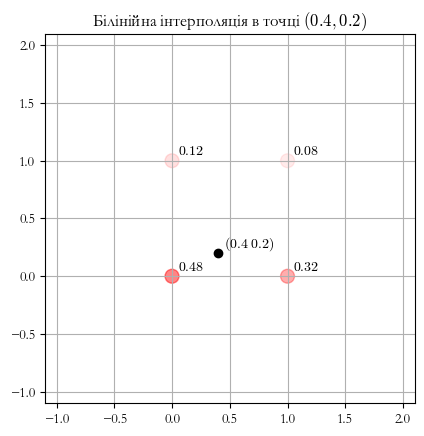
\includegraphics[width=0.5\textwidth]{img/bilinear-interpolation-1.png}
    \caption{
        Візуалізована білінійна інтерполяція в точці $(0{,}4,0{,}2)$ згідно формули~\eqref{e:blinterp}. 
        Значення в дробовій точці утворюється лінійною комбінацією значень у червоних точках на ґратці
        з коефіцієнтами, вказаними над точками.
    }
    \label{fig:bilinear-interp}
\end{figure}

Ідея статистики LBP \cite{ojala2002} полягає у використанні малої кількості тестових точок навколо пікселя для грубого опису поведінки його околу.
Побудуємо його з деяких простих міркувань.
Нехай все наше зображення містить лише одну текстуру.
У загальному випадку, статистика $T \colon K \to \R$ --- це скалярна функція, визначена для кожного пікселя зображення. 
При цьому, нехай $N_c \subset K$ --- множина координат пікселів, від значень яких залежить значення $T(c)$, $c \in K$. 
Вважатимемо, що $N_c$ будується для кожного пікселя однаково, на основі множини зсувів $R = \{r_i\} \subset \R^2$, $N_c = \{c' \mid c' - c \in R\}$, $0 = r_0 \in R$.
Тоді $T(c) = T(g_0, g_1, g_2, \dots, g_n)$, де $g_i = I(c_i)$, $c_i \in N_c$, при чому $g_0 = I(c)$, $\# N_c = n+1$.

LBP побудований в першу чергу з міркувань інваріантності відносно контрастності зображення.
Також, емпірично відомо, що значення ``центрального'' пікселя несе мало інформації, а важливішими є відносні значення рівнів.  
Зміна контрастності зображення математично описується монотонним перетворенням значень його пікселів: $I' = G \circ I$, $G \colon [0,255] \to [0,255]$, де $G$ -- строго монотонна.
У такому разі, 
\begin{equation*}
    T(g_0, g_1, \dots , g_n) = T(G(g_0), G(g_1), \dots , G(g_n)).
\end{equation*}
Одне з допустимих визначень має вигляд 
\begin{equation*}
    T = T(\{s(g_i - g_j) \mid 0\le i<j \le n\}), 
\end{equation*}
де $s(x) = \1(x \ge 0)$. 
Нехтуючи значенням центрального пікселя і відносними рівнями інших пікселів, можна спростити його до $T = T(\{s(g_i - g_0) \mid i=1,2,\dots,n\})$.

Найповніший опис околу за таких умов був би самим бінарним вектором $\tilde T(c) \in \{0,1\}^n$,
де $\tilde T(c)_k = s(g_k - g_0)$, $k=1,\dots,n$.
Бінарні вектори незручні у використанні у явному вигляді для комп'ютеризованих обчислень, проте, трактуючи їх як двійковий запис деякого числа, 
їх можна ототожнити із цілими числами. Математично така статистика формулюється як 
\begin{equation}\label{e:ojala-T}
    T(c) = T(s(g_1 - g_0), s(g_2 - g_0), \dots , s(g_n - g_0)) = \sum_{k=1}^n 2^{k-1}s(g_k-g_0),
\end{equation}

Перейдемо до побудови околу $N_c$. 
Розташування тестових точок $c_1,\dots ,c_n$ у 
радіальній симетрії відносно центру $c$ суттєво полегшить розробку інваріантного відносно обертання дескриптора $T$, хоча і не є обов'язковою умовою для цього.
Через скінченну роздільну здатність зображення було би недоцільно розглядати симетрію відносно повороту на довільно малий кут.
Тому, прийнято дискретизувати простір кутів на $P$ значень і розглядати симетрію лише відносно поворотів на кути кратні $\frac{2\pi}{P}$.
Ціле число $P$ називатимемо \emph{рівнем дискретизації}, а $\frac{2\pi}{P}$ -- \emph{кутом дискретизації}. 

У загальному випадку, тестові точки $N_c$ можуть бути розташовані на колах різних радіусів. 
На практиці прийнято розділяти точки різних радіусів на різні околи, тому вважатимемо, що усі точки $c_1,\dots ,c_n$ лежать на одному колі радіуса $R$.
Звідси, маємо, що всі точки мають бути рівномірно розподілені по колу з кроком, сумісним із $\frac{2\pi}{P}$.
Для визначенності, першу точку $c_1$ прийнято ставити праворуч від центру, за кутом 0 відносно горизонтальної осі, а наступні нумерувати за збільшенням кута.

Найчастіше, радіальний окіл $N_c$ радіуса $R$ та дискретизації $P$ має рівно $P$ точок і визначається як
\begin{equation}\label{e:circle}
    c_k = c_0 + R \cdot \begin{pmatrix} \cos \frac{2\pi (k-1)}{P} & \sin \frac{2\pi (k-1)}{P} \end{pmatrix}, \quad k=1,\dots,P
\end{equation}
Зауважу, що точки околу переважно мають дробові координати, тобто значення $I(c_k)$ мають обчислюватися шляхом білінійної інтерполяції за формулою~\eqref{e:blinterp}.

\begin{figure}[h]
    \begin{subfigure}{0.48\textwidth}
    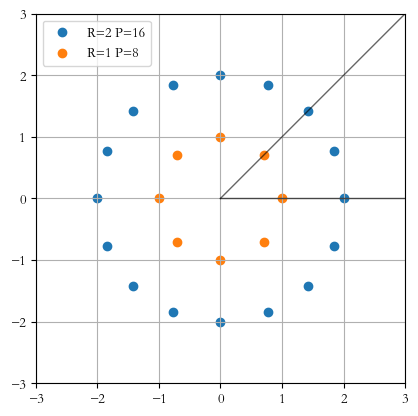
\includegraphics[width=0.9\linewidth]{img/clique-2.png} 
    \caption{
        Типовий окіл для обчислення інваріантної відносно обертання статистики із дискретизацією 8 або $\frac{\pi}{4}$. 
    }
    \label{subfig:clique-2a}
    \end{subfigure}%
    \hfill
    \begin{subfigure}{0.48\textwidth}
    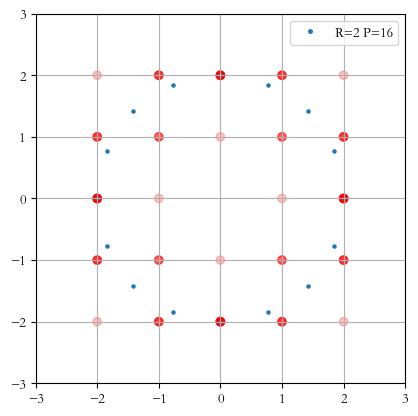
\includegraphics[width=0.9\linewidth]{img/clique-2-interp.png}
    \caption{
        Фактичні точки на ґратці, що приймають участь у обчисленні статистики на околі радіуса 2.
    }
    \label{subfig:clique-2b}
    \end{subfigure}
    
    \caption{}
    \label{fig:clique-2}
\end{figure}

\subsection{Узагальнений \(\mathrm{LBP}_{R,P}\)}\label{section1.1a}\hfill

Узагальнені LBP коди \cite{ojala2002} визначаються в точності згідно формули~\eqref{e:ojala-T} на околі~\eqref{e:circle}, покладаючи $n=P$.
При цьому $R$ та $P$ є гіперпараметрами, підбір яких є нетривіальною задачею.
Поширено використання векторної статистики $T = \begin{pmatrix}
    \mathrm{LBP}_{R_1,P_1} & \dots  & \mathrm{LBP}_{R_m,P_m}
\end{pmatrix}$. У такому випадку, $P$ може однозначно залежати від $R$ \cite{fastlbp2024}, або залишатись сталим для всіх радіусів \cite{huawudeng2004}.
За параметрів $R=1$, $P=8$ ми отримуємо статистику, близьку до першої версії статистики локальних бінарних шаблонів $\mathrm{LBP}_8$, у якій окіл визначається не на колі, а на 8-ми сусідніх пікселях.

На практиці, значення $P$ не може необмежено зростати: після $P=64$ числові значення $T$ виходять за межі діапазону значень типової цілочисленої змінної сучасних комп'ютерів довжиною в 64 біти, 
що робить околи більших розмірів недоцільними. У таких випадках доцільно розбивати більші околи на декілька менших, і працювати з вектором статистик відповідних околів,
що грубо відповідатиме конкатенації бітових векторів. 

На основі цього текстурного дескриптора часто будують інші, деякі з них перелічені далі.
Достатньо мале $P$ також означає, що похідний дескриптор $T' = F \circ T$ доцільно реалізовувати з допомогою обчислених заздалегідь таблиці пошуку у вигляді масиву, 
де індексами будуть можливі значення $T$.
Тоді, обчисленя $T'$ зводиться до обчислення $T$ та отримання значення цього масиву за індексом $T$, що часто є набагато швидшою операцією, ніж обчислення $T'$.
Розмір таблиці пошуку залежить від області визначення похідного дескриптора; 
для $F \colon \{0,\dots,2^P\} \to \{0,\dots,2^P\}$ та $P\le 64$ таблиця складатиметься з цілочисленних значень не більш, ніж int64, 
а отже матиме розмір $W_P$ не більше ніж $W_P = 2^P \cdot 8$ байтів. 
Для прикладу, $W_{32} \approx 34{,}3$ GB, що є непрактичним обсягом пам'яті, але $W_{24} \approx 135$ MB і $W_{16} \approx 0{,}5$ MB.

\subsection{Інваріантність відносно обертання у \(\mathrm{LBP}_{R,P}^{ri}\)}\label{section1.1c}\hfill

В основному, текстурні дескриптори розробляються у припущенні, що орієнтація текстур у тренувальних та тестових зображеннях співпадають.
Якщо орієнтація текстур довільна, то якість класифікації на основі цих дескрипторів стрімко падає. 
Очевидним рішенням буде доповнювати тренувальні дані синтетичними зображеннями, утвореними обертанням оригінальних. 
Іншим підходом буде використовувати в побудові дескриптора інваріантні статистики (напр. інваріантний LBP) чи 
``стерти'' інформацію про орієнтацію зі статистик чи з дескриптора (напр. з допомогою дискретного перетворення Фур'є). 
На практиці, точність класифікації суттєво покращується при перетворенні варіантних ознак на комбінацію інваріантних ознак, та ознак із інформацію про орієнтацію, наприклад з допомогою фільтрів Габора \cite{guo2010lbpv}. 

Нехай $\operatorname{rot}$ --- оператор циклічної перестановки елементів вектора,
\begin{equation*}
    \operatorname{rot} \begin{pmatrix}a_1 & a_2 & \dots  & a_P\end{pmatrix} = \begin{pmatrix}a_P & a_1 & \dots  & a_{P-1}\end{pmatrix}.
\end{equation*} 
Введемо відношення еквівалентності $A\sim B \iff \exists k: A = \operatorname{rot}^k B$, де $A,B \in \{0,1\}^P$.
Зверну увагу, що $\operatorname{rot}^P A = A$ та $\operatorname{rot}^{P-k} \operatorname{rot}^k A = A$.

За цим відношенням еквівалентності розіб'ємо простір значень бінарного вектора $A = \begin{pmatrix}
    s(g_1 - g_0) & s(g_2 - g_0) & \dots  & s(g_P - g_0)
\end{pmatrix}$, з якого далі обчислюється статистика $\mathrm{LBP}_{R,P}$. 
Циклічна перестановка цього вектора відповідає циклічній перестановці індексів точок $c_1, c_2, \dots , c_P$ околу навколо $c_0$, визначеного у~\eqref{e:circle} 
(що у свою чергу моделює обертання зображення на кут, кратний куту дискретизації).
Інваріантний відносно обертання дескриптор $\mathrm{LBP}^{ri}$ обчислюється як найменше числове значення $\mathrm{LBP}_{R,P}$ серед таких околів,
тобто найменше числове значення серед циклічних перестановок бінарного вектора $A \in \{0,1\}^P$,
\begin{equation*}
    \mathrm{LBP}^{ri}_{R,P} = \min_{0\le k < P} \mathrm{LBP}_{R,P} \left( \operatorname{rot}^k A \right).
    % = \min_{0\le k < P} \sum_{i=1}^P s(g_{(i + k) \operatorname{mod} P} - g_0) 2^{(i + k - 1) \operatorname{mod} P}.
\end{equation*}
Ця величина також називається (лексикографічно) мінімальним обертанням рядка $A$ або словом Ліндона.   

Окрім набуття інваріантності, оператор $\mathrm{LBP}^{ri}_{R,P}$ також має меншу область значень, ніж $\mathrm{LBP}_{R,P}$.
Позначимо клас еквівалентності $A$ за відношенням еквівалентності, породженим прообразом $\mathrm{LBP}^{ri}_{R,P}$, як $[A]$.
Тобто, $A \sim A' \iff \mathrm{LBP}^{ri}_{R,P} A = \mathrm{LBP}^{ri}_{R,P} A'$.
Розмір класів еквівалнетності не сталий і залежить від періоду вектора. 
Наприклад, $\# [\texttt{00000000}] = 1$, $\# [\texttt{01010101}] = \# \{01010101,10101010\} = 2$, $\# [00100100] = 8$.

Назвемо вектор періодичним з періодом $0<k\le P$, якщо $\operatorname{rot}^k A = A$ і $k$ є найменшим таким числом.
Вектор з періодом $P$ назвемо неперіодичним.
Зауважу, що не всі періоди можливі. Нехай $d=\operatorname{gcd}(k,P)$ -- найбільше спільне кратне, $d\le k < P$. 
Існують $r,s\in \Z$ такі, що $d=rk+sP$. Тоді $\operatorname{rot}^d A = \operatorname{rot}^{rk+sP} A = \operatorname{rot}^{rk} A = A$.
Але $k$ -- найменше таке число, тобто $k \le d$, звідки маємо $d=k$. Таким чином, періоди -- це дільники $P$.
Зрозуміло, що клас еквівалентності $k$-періодичного вектора тоді має розмір $k$, проте кількість різних $k$-періодичних векторів нетривіальна.
Проте, зрозуміло, що $\# \{A\in \{0,1\}^P \mid \operatorname{rot}^k A = A\} = \operatorname{gcd}(k,P)$.  

Тоді, за лемою Бернсайда, $\mathrm{LBP}^{ri}_{R,P}$ приймає $N^{ri}_P = \frac{1}{P}\sum_{k=1}^P 2^{\operatorname{gcd}(k,P)}$ різних значень. 
Ця величина природним чином є кількістю різних орбіт дії групи $\Z/P\Z$ на $\{0,1\}^P$, а також, кількістю різних двоколірних намист довжини $P$.
Асимптотично, $N^{ri}_P \sim \frac{2^P}{P} + o(2^P)$. 
Для прикладу, $N^{ri}_8 = 36$, $N^{ri}_{16} = 4116$, $N^{ri}_{24} = 699252$

\subsection{Рівномірний \(\mathrm{LBP}_{R,P}^{riu}\) та інші}\label{section1.1d}\hfill

У подальших дослідженнях \cite{ojala2002} було помічено, що для деяких застосувань та малих радіусів найчастіше (90\% та більше) трапляються так звані ``рівномірні'' (uniform) послідовності, 
в яких є чітка межа між одиницями та нулями, тобто не більш ніж 2 переходи від 0 до 1 чи назад. 
Тобто, мінімальне представлення бінарного вектору $A$ матиме $u$ нулів, за якими йдуть $P-u$ одиниць.
Після цього спостереження розроблено ``рівномірний'' $\mathrm{LBP}^{riu}_{R,P}$, 
який ставить у відповідність рівномірному вектору кількість одиниць від $0$ до $P$, а нерівномірному -- спеціальне значення $P+1$.
$\mathrm{LBP}^{riu}_{R,P}$ приймає $P+2$ різних значень.

Наше дослідження \cite{fastlbp2024} базується на доробку Benjamin Woodhams, долученого до \cite{lee2025integrated}, і використовує саме цей варіант дескриптора LBP.
Його доцільність залишається дискусійним питанням, бо у випадку великих зображень та великих радіусів 
частка рівномірних околів стрімко зменшується.

\begin{figure}[h]
    \centering
    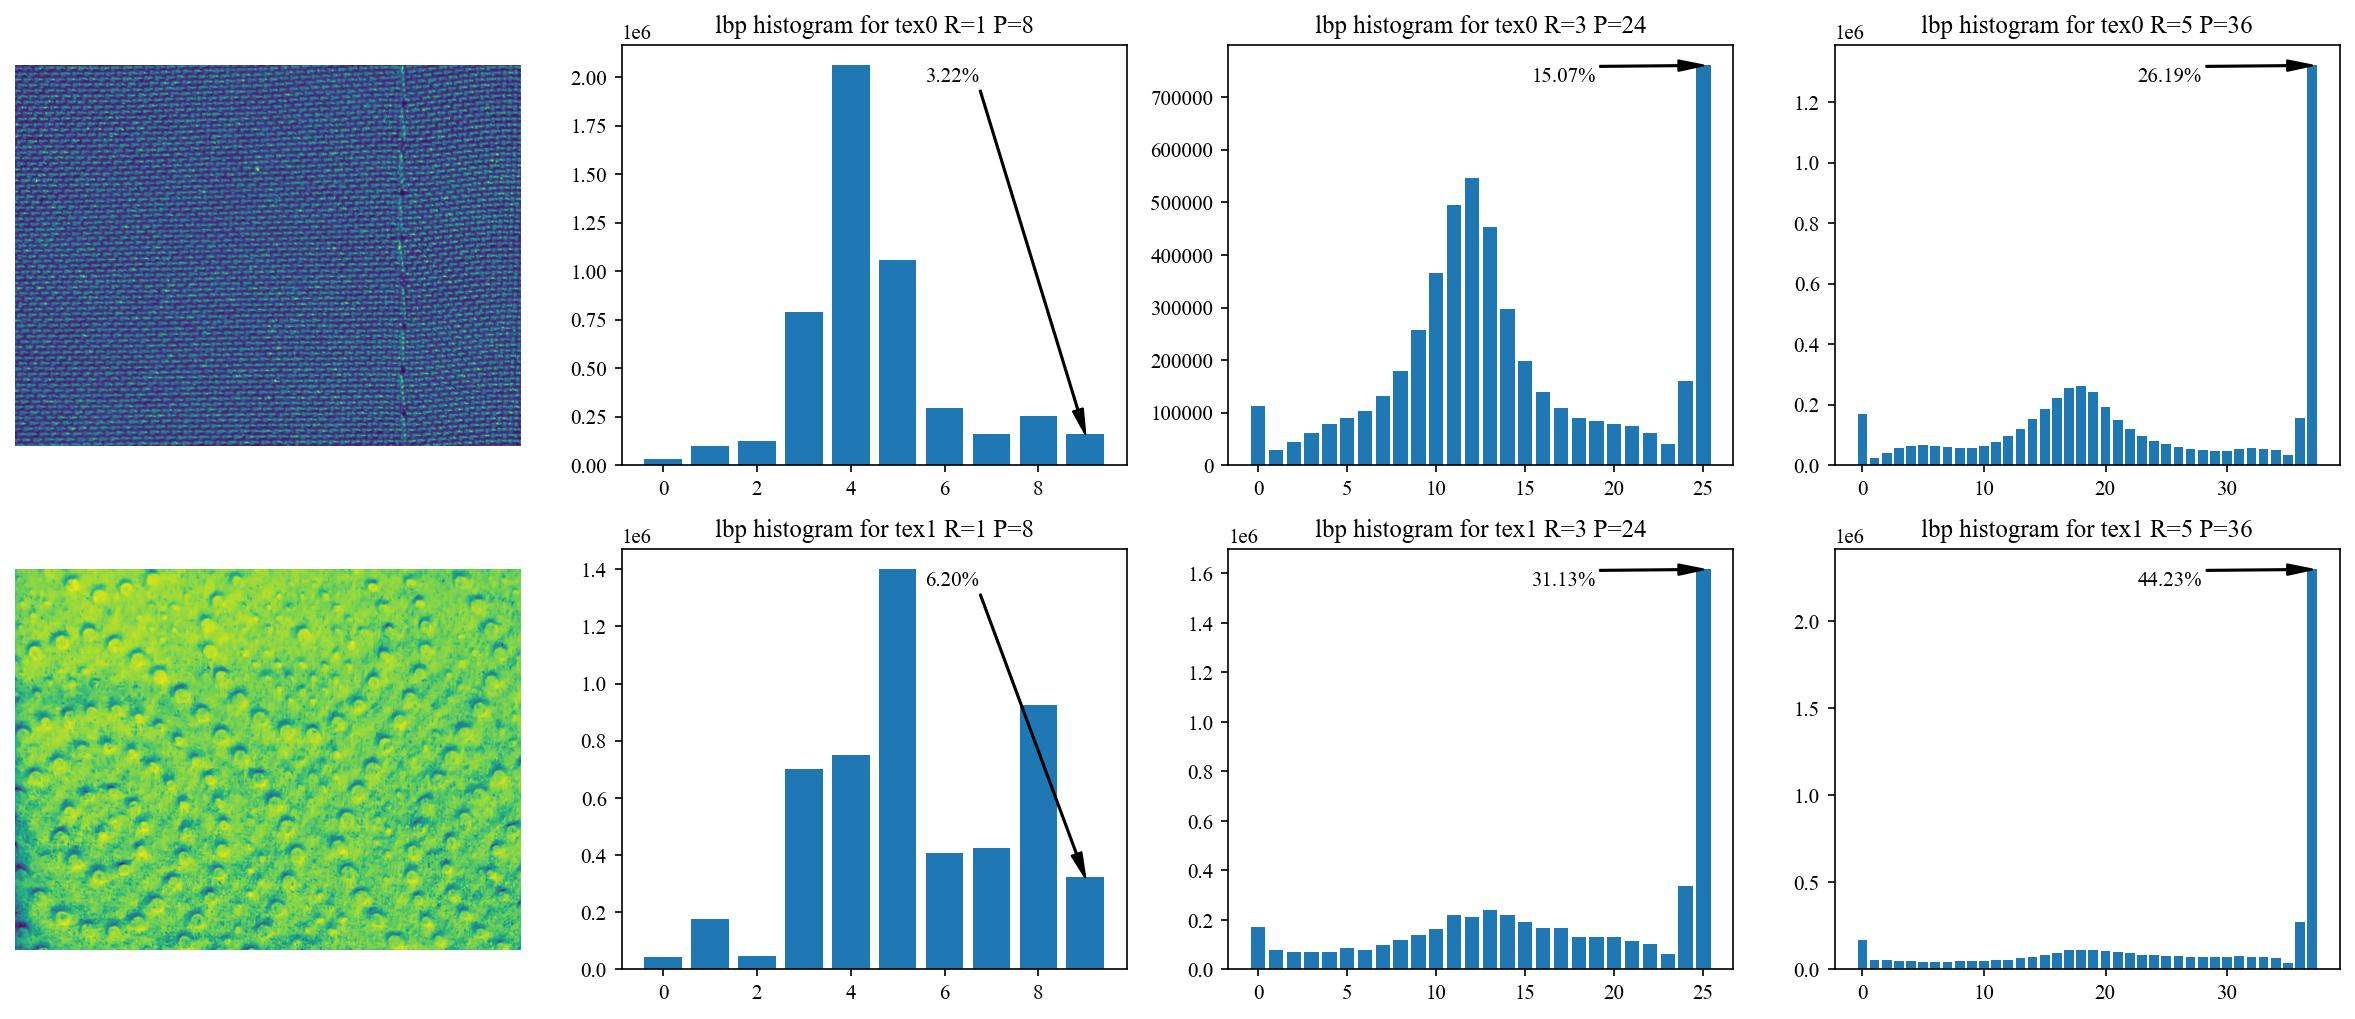
\includegraphics[width=0.99\textwidth]{img/cloth-hist-lbpu.jpg}
    \caption{
        Гістограми LBP із різними $R$ та $P$ для двох текстур.
        Демонструється збільшення кількості нерівномірних околів зі збільшенням $R$.
    }
    \label{fig:cloth-hist-lbpu}
\end{figure}

Інший цікавий підхід полгає у застосуванні амплітуди дискретного перетворення Фур'є (DFT) LBP кодів у якості ознак \cite{arof1998, haley1999}.
Відомо, що DFT вектора не змінюється від його циклічних перестановок. 
Більше того, через симетричність амплітуди DFT відносно середини послідовності, достатньо зберігати лише половину координат, що зменшує кількість ознак. 

% =============================================



\section{Текстура як розподіл}\label{section1.2}\hfill

Розглянемо деяку статистику $T = T(c)$, визначену в кожному пікселі, що залежить від значень зображення у точках околу $N_c$ навколо цього пікселя.
Припускаємо, що зображення можуть містити лише одну текстуру, тобто текстура гомогенна.
Розглядатимемо текстуру як певний розподіл статистики $T$ на зображенні. 
За цієї гіпотези, візуально різні текстури матимуть різні розподіли $T$.
Ми прагнемо описати ці різні невідомі розподіли вектором параметрів, який далі можна використовувати як вектор ознак у задачі класифікації.

\subsection{Текстура як розподіл одного дескриптора}\label{section1.2a}\hfill

Гарною оцінкою розподілу буде гістограма значень $T$ на зображенні, вважаючи спостереженнями значення $T(c), \; c \in K$ для кожного пікселя~$c$ із координатами з множини координат $K$.
Ми також нехтуватимемо залежністю між значеннями $T$ в сусідніх пікселях, вважатимемо значення $T$ незалежними один від одного, і однаково розподіленими на зображенні.
Працюватимемо в імовірнісному просторі $(\Omega, \mathcal F, \mu)$.
Маємо незалежні однаково розподілені випадкові величини 
\[ T_c \colon \Omega \to D, \quad c \in K, \quad T_c \sim F \] 
із законом розподілу (функцією розподілу) $F \colon D \to [0;1]$, де $D = \{T_{\min},\dots,T_{\max}\} \subset \Z$.
При цьому вважаємо $T_{\min}, T_{\max}$ відомими; зазвичай $T_{\min} = 0$, $T_{\max} < 2^{64}$.

Емпірична функція розподілу $\hat F(d) = \sum_{c\in K} \1\{\ T_c \le d \}$
дає гарну (консистентну та асимптотично нормальну) оцінку справжньої функції розподілу $F(d) = P(T \le d)$.
Нам буде зручніше працювати із імовірностями окремих значень $D$, $f \colon D \to [0;1]$, $f(d) = P(T = d)$.
При цьому відповідною оцінкою $f$ буде 
\[\hat f(d) = \frac{1}{\# K}\sum_{c\in K}\1\{T_c = d\} = \frac{\hat\nu_d}{\# K}.\]

Послідовність $H = \{ \hat \nu_d, \; d\in D \}$ називатимемо \textit{гістограмою} $T$ на зображенні.
Послідовність $H_1 = \{ \hat \nu_d / \# K, \; d\in D \} = \{\hat f(d), \; d\in D\}$ називатимемо нормованою гістограмою, або вектором відносних частот.

Зауважу, що для багатьох дескрипторів складно ввести змістовний лінійний порядок на області значень. 
Наприклад, значення дескрипторів $\mathrm{LBP}_{R,P}$ та $\mathrm{LBP}^{ri}_{R,P}$ є природнім числовим представленням бінарного вектора, що відповідає лексикографічному порядку для цих бінарних векторів.
Малі зміни у вихідному векторі можуть привести до великих змін у його значенні (наприклад, бітфліп на старших позиціях).
Враховуючи сенс дескрипторів, на множині значень можна було би ввести квазіпорядок домінування, який би краще відобразив її структуру, проте це ускладнило би визначення функції ймовірності дескриптора.
Інтуітивно, це означає, що статистичні процедури потрібно вводити незалежно від способу упорядкування множини значень, 
а також підтверджує доречність частішого використання дискретної щільності ймовірності замість функції імовірності.

Одним з найбільш поширених підходів є розглядати розподіл $T$ як \textit{мультиноміальний}. 
У цьому випадку параметром розподілу буде вектор $\Theta = \{p_d, \; d\in D\}$, тобто імовірності кожного значення $T$.
Нормована гістограма буде особливо гарною оцінкою, $\hat \Theta = \{\hat f(d), \; d\in D\} = H_1$.
Більша кількість параметрів не має сенсу за умови незалежності $T_c$, а менша потребує нетривіального підбору моделі.
Область значень дескриптора іноді ділять на інтервали $D = \sqcup_{g\in G} D_g$.
Поділ на інтервали стає необхідним, якщо кількість пікселів (спостережень) співрозмірна або менша за кількість різних значень дескриптора, 
або використовуються неперервні текстурні дескриптори, наприклад, скалярні статистики дескриптора GLCM, перелічені у \cite{belsare2015}.

Отже, вектором ознак текстури згідно дескриптора $T$ може бути його гістограма $H$,
\begin{equation*}
    \xi = \{\hat\nu_d, \; d\in D\}.
\end{equation*}

\subsection{Текстура як розподіл декількох дескрипторів}\label{section1.2b}\hfill

Один дескриптор нечасто дає достатньо інформації для того, щоб відрізнити текстури між собою, особливо в роботі із спорідненими текстурами, 
такими як різні стани одного матеріалу, чи різні підтипи одного типу біологічної тканини.
З іншого боку, різні текстури можуть проявляти свої особливості у різних просторових масштабах.
Відповідно, часто використовуються набори різних статистик $T^m$ (наприклад, LBP із різними параметрами $R$ та $P$).
Особливо інформативними вважаються моделі, побудовані на сумісних розподілах дискретних статистик разом з неперервними \cite{guo2010lbpv}.

Нехай статистики $T^m$ мають області значень $D^{(m)}$. 
У загальному випадку, сумісний розподіл всіх $T^m\colon\ \Omega \to D^{(m)}$, $m=1,\dots,M$ оцінюється багатовимірною гістограмою. 
У мультиноміальній моделі, кількість параметрів сумісного розподілу зростатиме як добуток потужностей області значень $\prod_{m=1}^M \# D^{(m)}$, або відповідних розбиттів областей значень.
Розглядати сумісні розподіли багатьох статистик недоцільно, бо із зростанням кількості статистик експоненційно зростає кількість класів гістограми, 
збільшується довжина вектора ознак, зменшуючи кількість спостережень кожного класу, та статистичну значущість висновувань.
Тому, дескриптори $T^m$ часто розглядають як незалежні, від чого кількість параметрів сумісного розподілу зростатає не як добуток, а лише як сума $\sum_{m=1}^M \# D^{(m)}$.

Отже, вектор ознак текстури згідно декількох незалежних дескрипторів $T^m$ можна утворити конкатенацією декількох гістограм,
\begin{equation*}
    \xi = \bigsqcup_{m=1}^M \{\hat \nu^{(m)}_d, \; d\in D^{(m)}\}.
\end{equation*}



% ================================




\section{Класифікація текстур}\label{section1.3}
% Майборода. Непараметрична статистика

% один дескриптор
Нехай спостерігаються зображення $I \colon K \to \{0,\dots,255\}$,%
\footnote{$K$ -- множина координат зображення, одна для всіх зображень. Вважаємо, що всі зображення одного розміру.}
кожне з яких містить одну з $S$ різних текстур, які позначатимемо номерами $1,\dots,S$.
Текстуру, що відповідає зображенню, позначатимемо $\kappa(I)$.
Використовуємо один текстурний дескриптор $T$ із областю значень $D = \{T_{\min},\dots,T_{\max}\} \subset \Z$ і обчислюємо його значення в кожному пікселі. 
Зображенню відповідає набір з $\# K$ значень який вважатимемо випадковою величиною
\[ T(I) = \left(T(I,c),\; c\in K\right), \quad T(I)\colon \ \Omega \to D^{\# K}, \]
при цьому $T(I,c)$ -- незалежні за $c$ й однаково розподілені за законом~$F$.
Припускаємо, що текстура характеризується \emph{розподілом} текстурного дескриптора $T$, тобто розподіл $F = F_{\kappa(I)}$ залежить від $\kappa(I)$.
Задачею є деяким чином оцінити невідоме $\kappa(I)$ за спостереженими $T(I,c)$.

% % багато дескрипторів
% Нехай спостерігаються зображення $I \colon K \to \{\overline{0,255}\}$, кожне з яких містить одну з $S$ різних текстур, які позначатимемо номерами.
% Текстуру, що відповідає зображенню, позначатимемо $\kappa(I)$.
% Використовуємо $M$ незалежних текстурних дескрипторів $T^m$ і обчислюємо їх значення в кожному пікселі. 
% Для зручності, припускаємо, що всі $T$ мають одну область значень $D = \{\overline{T^m_{\min}, T^m_{\max}}\} \subset \Z$.
% Кожному зображенню відповідає набір з $\# K$ значень кожного з $M$ дескрипторів, який вважатимемо випадковою величиною
% \[ T^m(I) = \left(T^m(I,c),\; c\in K\right) \colon \Omega \to D^{\# K}, \]
% при цьому $T^m(I,c)$ -- незалежні за $m$ та $c$, та однаково розподілені за законом~$F_m$ ($T^m$ незалежні та по-різному розподілені).
% Припускаємо, що текстура характеризується \emph{розподілами} текстурних дескрипторів $T^m$, тобто розподіли $F_m$ залежать від $\kappa(I)$.
% Задачею є деяким чином оцінити невідоме $\kappa(I)$ за спостереженими $T^m(I,c)$.

Припустимо, що ми також маємо навчальну вибірку, тобто для певної кількості інших зображень $I^t$ відомі дійсні значення $\kappa(I^t)$. 
Для деякого статистичного критерію близкості розподілів із статистикою~$X$ та критичною областю~$X_c$ можна побудувати серію критеріїв~$X^{(s)}$ 
для оцінки близкості до кожної відомої текстури і на їх основі побудувати класифікатор.

\subsection{Критерій $\chi^2$}\label{section1.3a}\hfill
% https://stats.stackexchange.com/questions/1047/is-kolmogorov-smirnov-test-valid-with-discrete-distributions
% todo: normality test?????

Припустимо, що використовуємо один текстурний дескриптор $T$.
У~кожному пікселі $\P(T = d) = p^{(s)}_d$, і при цьому значення $T$ не залежить від значень у інших пікселях.
Тоді, розподіл частот $\left(\nu_d, d\in D\right)$ є мультиноміальним із імовірностями~$p^{(s)}_d$ та 
кількістю спостережень рівною кількістю пікселів на зображенні $\# K$, $\sum_{d}\nu_d = \# K$. 
Закон розподілу має наступний вигляд
\begin{equation*}
    f_s(\{ \nu_d \}) = \frac {\Gamma (\sum_{d}\nu_{d}+1)}{\prod_{d}\Gamma (\nu_{d}+1)} \prod (p^{(s)}_d)^{\nu_d}.
\end{equation*}

Нехай $e^{(s)}_d, d \in D$ -- усереднена частота появи значення~$d$ дескриптора~$T$ на зображеннях, яким відповідає відома текстура~$s$
($e^{(s)}_d = \# K \cdot p^{(s)}_d$), а $\nu_d$ -- частота появи значення на зображенні, текстуру якого ми класифікуємо.

Нульовою гіпотезою вважаємо те, що розподіли $T$ для текстури $s$ та на оцінюваному зображенні рівні.
Якщо припустити, що за нульової гіпотези спостережувані частоти є нормально розподіленими навколо очікуваного значення, $\nu_d \sim \mathcal N(e^{(s)}_d, )$, то можна розглядати статистику
\begin{equation*}\label{e:chi2crit}
    X(\vec \nu,\vec e^{(s)}) = \sum_{d \in D} \frac{\left(\nu_d - e^{(s)}_d\right)^2}{e^{(s)}_d} \longrightarrow \chi^2_{\# D - 1}.
\end{equation*}
Для рівня значущості $\alpha$ критичним значенням буде, відповідно, квантиль рівня $1-\alpha$ розподілу $\chi^2$ із $\# D - 1$ степенями свободи.
Зауважу, що на практиці гіпотеза нормальності спостережуваних частот може не підтверджуватись.

Примітивний класифікатор може мати вигляд
\begin{equation*}\label{e:chi2classifier}
    g(I) = \arg \min_{s} X^{(s)},
\end{equation*} 
що мінімізує ймовірність помилки, враховуючи односторонність критерію, та еквівалентно пошуку найближчого $\vec p^{(s)}$ до $\vec \nu$ у $L^2$ сенсі.

\subsection{Статистичний критерій log-правдоподібності}\label{section1.3b}\hfill

Іншим поширеним критерієм близкості розподілів є критерій відношення лог-правдоподібності, або G-test.
Статистика критерію має вигляд%
\begin{equation*}\label{e:gtest-1}
    G(\vec \nu,\vec e^{(s)}) = 2\sum_{d \in D} \nu_d \log \frac{\nu_d}{e^{(s)}_d} \longrightarrow \chi^2_{\# D - 1}.
\end{equation*}
$G$ також є відстанню Кульбака--Ляйблера між гістограмами $\nu_d$ та $e^{(s)}_d$. 

% потужність порівняно з \chi^2?

Класифікатор тоді може мати вигляд
\begin{equation}\label{e:gtest-classifier-1}
    g(I) = \arg \min_s  \sum_{d \in D} \nu_d \log \frac{\nu_d}{e^{(s)}_d}
\end{equation}
або, еквівалентно, 
$g(I) = \arg \max_s  \sum_{d \in D} \nu_d \log e^{(s)}_d.$
% \begin{equation*}\label{e:gtest-classifier-2}
%     g(I) = \arg \max_s  \sum_{d \in D} \nu_d \log e^{(s)}_d.
% \end{equation*}

\subsection{Класифікація за $k$ ближніми сусідами}\label{section1.3c}\hfill

Попередні два способи фактично визначають дещо схоже на відстань на просторі зображень і класифікують за близкістю до центру класів.
Точнішим способом є класифікація за $k$ ближніми у деякому сенсі сусідами, де передбачений клас визначається як найчастіший серед сусідів.
Таким чином можна уникнути усереднення гістограм і покращити точність класифікації у випадку, коли текстура може мати різні представлення у вигляді гістограм.
Іншою перевагою є те, що при використанні залежного від обертання дескриптора, для тренування можна використовувати також повернуті варіанти зображень, що дозволить класифікувати зоображення із різними орієнтаціями.



%%


\newpage

\chapter{Практичні результати}\label{chapter2}

\section{Експериментальні результати}\label{section2.1}

Для перевірки гіпотез на практиці було написано набір Python скриптів.
За основу взято відомий датасет текстур Бродатца \cite{brodatz} із фотографіями у відтінках сірого у однорідному освітленні.
Цей датасет використовується в тому числі для сумісності результатів із іншими науковими роботами.
Спочатку з оригінального датасету утворено тренувальні та тестові вибірки у потрібному форматі.
Далі проведено перевірку деяких сформульованих в роботі статистичних гіпотез для цієї вибірки.
Потім підготовлено статистичну модель для класифікації текстур декількома методами і оцінено їх ефективність.

\subsection{Підготовка даних}\label{section2.1a}

\begin{figure}[h]
    \centering
    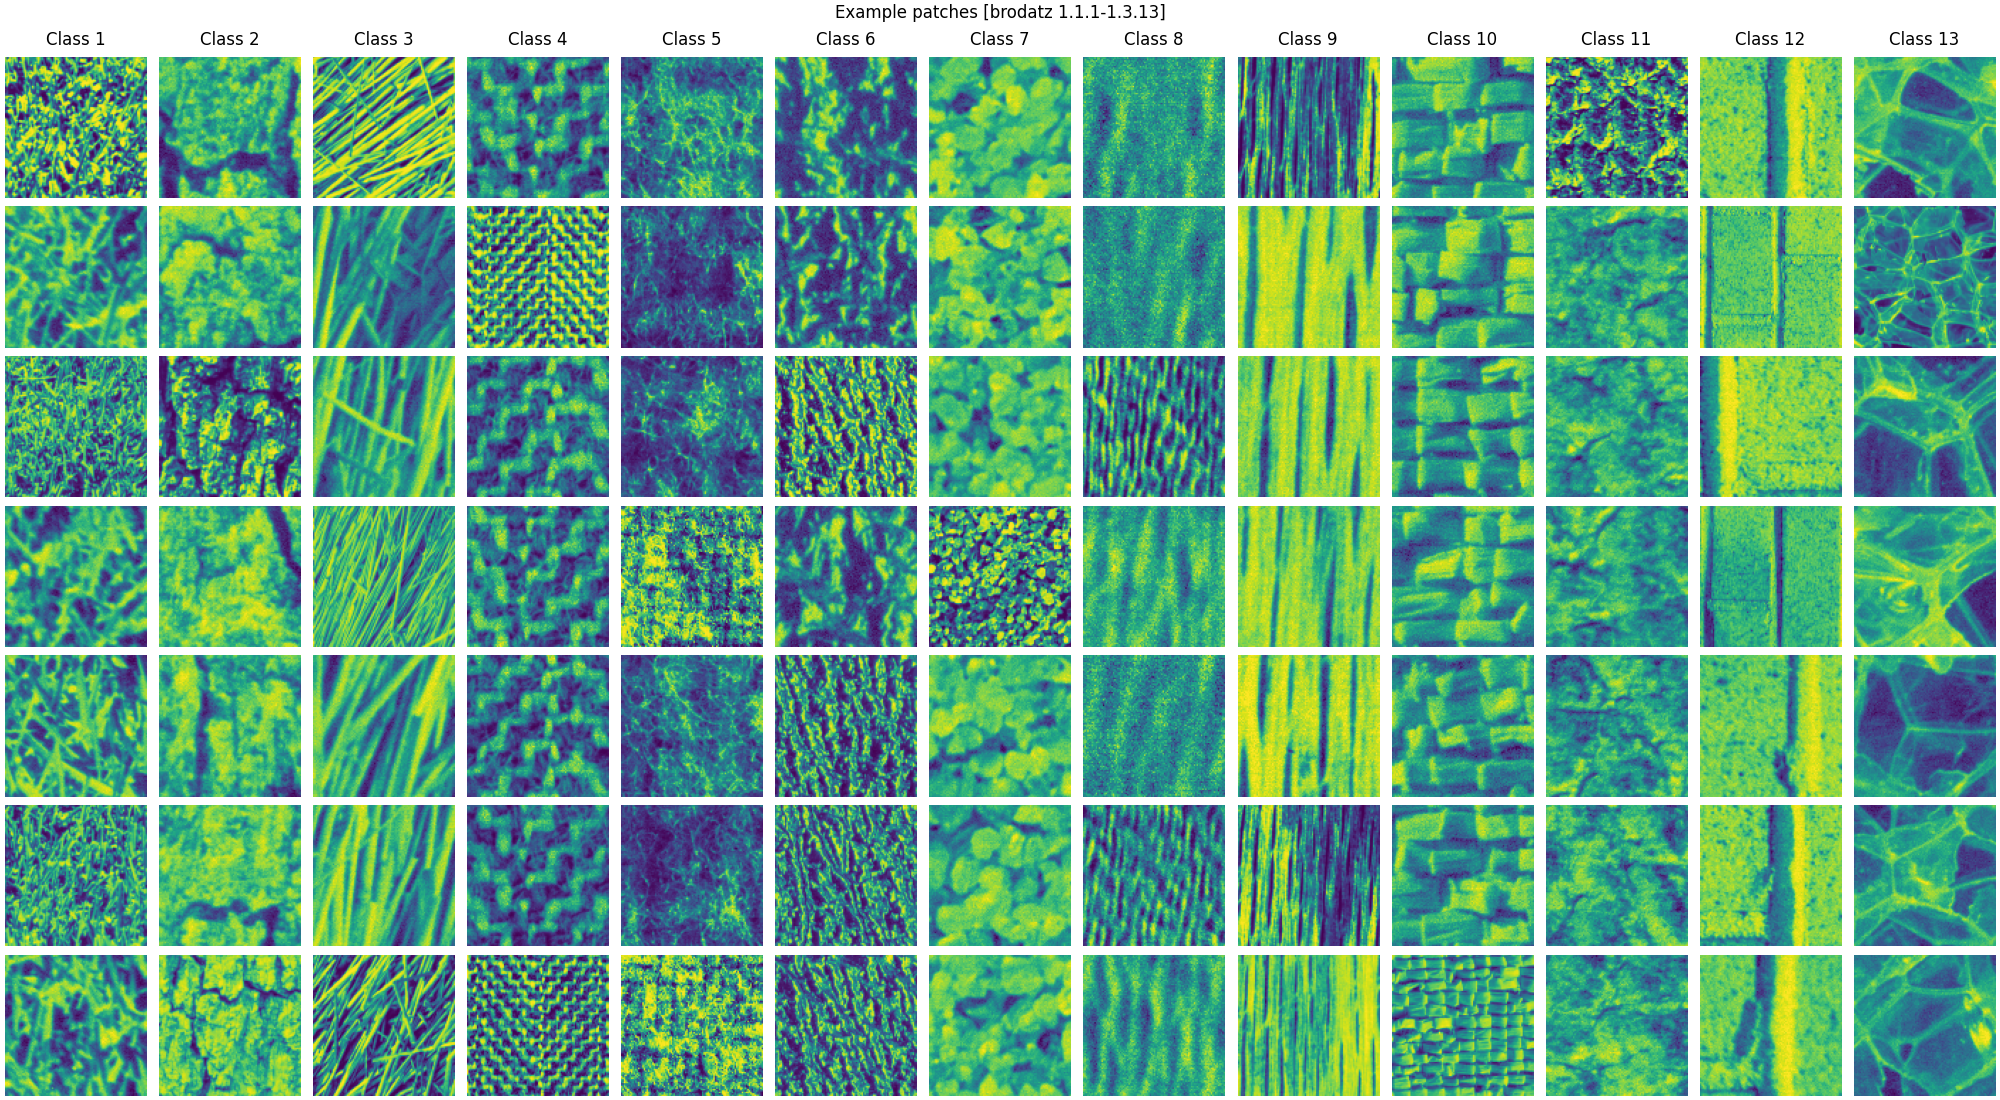
\includegraphics[width=0.99\textwidth]{img/example_classes.png}
    \caption{
        Приклад патчів 100x100 у відтінках сірого, утворених з датасету текстур Бродатца; для кожного з типів текстур у наборі.
        Візуалізовано у псевдокольорах.
    }
    \label{fig:brodatz-showcase}
\end{figure}

У роботі використано перші три частини датасета Бродатца, які містять фотографії текстур у відтінках сірого у великому наближенні, всього 39 різних фотографій.
Датасет включає як однорідні та регулярні текстури (цегла, тканина), так і псевдорегулярні (дерево, кора, трава, сіно, шкіра). 
Кожна частина складається з 13-ти фотографій різних текстур (природних та штучних), при чому послідовність текстур повторюється між частинами. 
Зображення у перших двох частинах мають розміри 512 на 512 пікселів. 
Третя частина містить фотографії в іншому масштабі та у розмірі 1024 на 1024 пікселів.
Оригінальні фотографії розрізано на неперетинні квадратні частини (патчі) розміром 100 на 100 пікселів (ігноруючи залишкові пікселі).
Кожному патчу призначено дві мітки: номер текстури (1-13), та номер фотографії цієї текстури, з якого патч походить (1-3).

Таким чином, робоча вибірка містить по 350 патчів з першої та другої частин, і 1300 патчів з третьої частини; всього 1950 елементів вибірки.
Всі текстури представлені у вибірці збалансовано, кожна має по 150 представників.

\subsection{LBP дескриптори}\label{section2.1b}

У якості дескрипторів у роботі будуть дескриптори LBP із різними параметрами R та P, у стандартному та "рівномірному" варіантах.
Для сумісності результатів із попередніми дослідженнями \cite{ojala2002,fastlbp2024}, обрано наступні параметри:
(R=1,P=8), (R=2,P=12), (R=1,P=8, "рівномірний"), (R=2,P=12, "рівномірний"), (R=3,P=24, "рівномірний"), (R=5,P=36, "рівномірний").
Кожному дескриптору відповідає вектор ознак, що обчислюється як гістограма значень дескриптора на зображенні (послідовність частот $\nu^{(T)}_d(I)$).
Для кожного патчу обчислено всі вектори ознак (наприклад, Рис. \ref{fig:example-features}).

\begin{figure}[h]
    \centering
    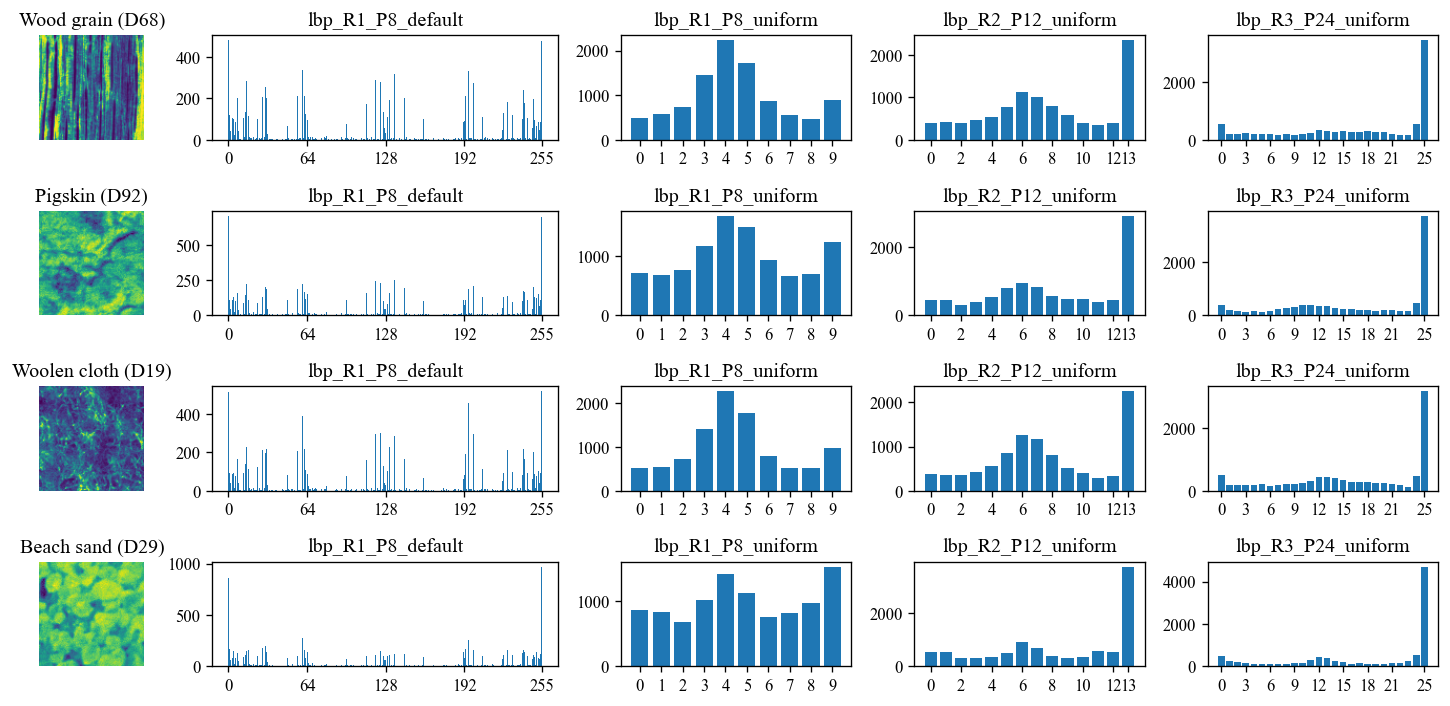
\includegraphics[width=0.99\textwidth]{img/example_features.png}
    \caption{
        Приклад деяких векторів ознак (гістограм) для деяких патчів
    }
    \label{fig:example-features}
\end{figure}

Для не-рівномірних дескрипторів стає суттєвою невелика кількість пікселів у патчі 100x100.
Дескриптор R1P8 приймає 256 можливих значень і багато з них приймає рідко -- гістограма цього дескриптора містить медіанно 33\% частот менше 5, мінімально 15\% .
Дескриптор R2P12 приймає 4096 можливих значень і практично всі з них приймає рідко -- медіанно 92\% частот менше 5, мінімально 90\% .

Малі значення частот викривляють результати вищезгаданих статистичних тестів і збільшують залежність результату від точності обчислень.
Має сенс розділити множину значень дескриптора на $B$ рівних інтервалів, обираючи $B$ таким чином, щоб кількість малих частот була не більше, наприклад, 5\% \cite{ojala2002}.

Для мого датасету шляхом перебору виявилося, що 64 це гарна кількість інтервалів для R1P8. 
Це відповідає об'єднанню початкових 256 інтервалів по 4. 
За цих умов не більше 1,6\% нових інтервалів матимуть менш ніж 5 спостережень.
Для R2P12 гарною кількістю інтервалів виявилось 90. 
Це відповідає об'єднанню початкових 4096 інтервалів по 46. 
За цих умов не більше 5\% нових інтервалів матимуть менш ніж 5 спостережень.

Значення у гістограмах, що відповідають "рівномірним" дескрипторам LBP, не були об'єднані в інтервали, 
оскільки кількість різних значень на порядки менша за кількість спостережень і проблем із малими частотами не було.

\subsection{Статистична гіпотеза нормальності відхилень гістограми}\label{section2.1c1}

Для цього обчислено відхилення кожного вектору ознак від середнього значення серед інших векторів цього класу текстури.
Використано критерій нормальності Шапіро-Вілка (\verb|scipy.stats.shapiro|) окремо для кожної координати вектору ознак із значущостю 0,05.
Обчислено частку ймовірно не-нормально розподілених координат вектора у кожному класі текстур, а потім медіану по всім класам текстур.

Отримані результати зображено на Рис. \ref{fig:normaltest}. 
Бачимо, що в цілому не можемо припускати, що гістограми розподілено нормально навколо середньої у кожному класі.
Цікаво, що нормальність суттєво вища для ознак, утворених розбиттям гістограми на інтервали (reb\_hist\_R1\_P8\_d та reb\_hist\_R2\_P12\_d).

\begin{figure}[h]
    \centering
    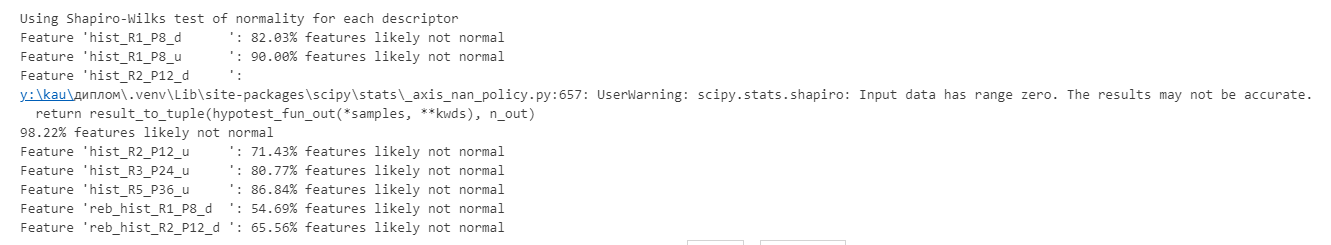
\includegraphics[width=0.9\textwidth]{img/normality-test.png}
    \caption{
        Результати застосування критерію нормальності 
    }
    \label{fig:normaltest}
\end{figure}

Також перевірено нормальність враховуючи те, що патчі були взяті з різних зображень із різними масштабами (Рис. \ref{fig:normaltest-subsets}).
Бачимо, що всередині підмножини вибірки нормальність значно вища.
Це може свідчити про те, що у загальній вибірці всередині класу маємо деяку суміш розподілів.
Таким чином, патчі з різних зображень одного типу текстури ймовірно мають суттєво різні розподіли, що необхідно враховувати при проєктуванні класифікаторів.
Ця гіпотеза буде перевірена глибше у наступних розділах.

\begin{figure}[h]
    \centering
    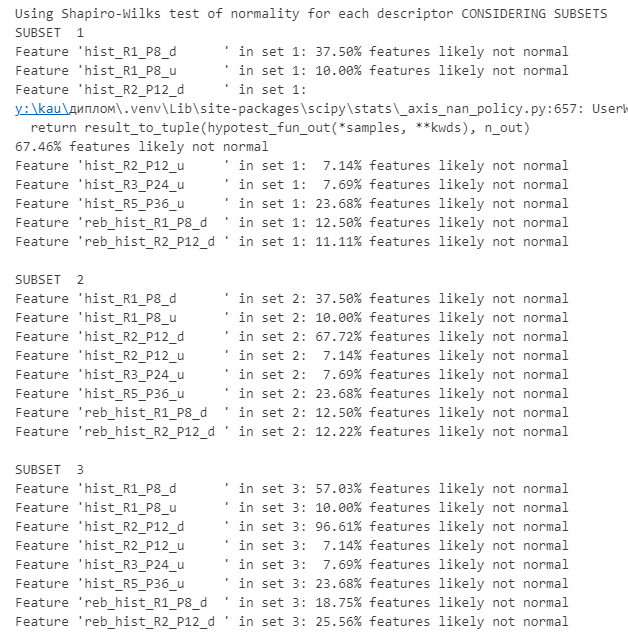
\includegraphics[width=0.5\textwidth]{img/normality-test-subsets.png}
    \caption{
        Результати застосування критерію нормальності із врахуванням підмножин вибірки
    }
    \label{fig:normaltest-subsets}
\end{figure}


\subsection{Статистична гіпотеза близькості середніх розподілів}\label{section2.1c2}

Якщо моделювати текстуру як деякий розподіл, то класифікація текстур може виконуватись за близькістю 
спостережуваної гістограми до інших, еталонних гістограм. 
Для використання статистичних критеріїв близькості розподілів ми припускаємо, 
що спостережувана гістограма сама є реалізацією деякого розподілу, 
наприклад нормального розподілу із центром у середній гістограмі певного класа текстури.
У попередньому пункті перевірено, наскільки доцільно вважати цей розподіл нормальним.
У цьому пункті перевіримо, чи достатньо суттєво відрізняються середні гістограми класів текстур, щоб вважати, 
що відповідні текстури моделюються різними розподілами.

Для середніх гістограм кожної пари класів текстур було обчислено критерій близькості розподілів відношення log-правдоподібності (\verb|scipy.stats.power_divergence| із \verb|lambda_='log-likelihood'|). 
Спершу разом для всіх патчів датасету \ref{fig:distr-sim-all}, а потім враховуючи зображення, з якого походить патч \ref{fig:distr-sim-subsets}. 
В обох випадках прийнято рівень значущості 0,05. 

\begin{figure}[h]
    \begin{subfigure}{0.48\textwidth}
    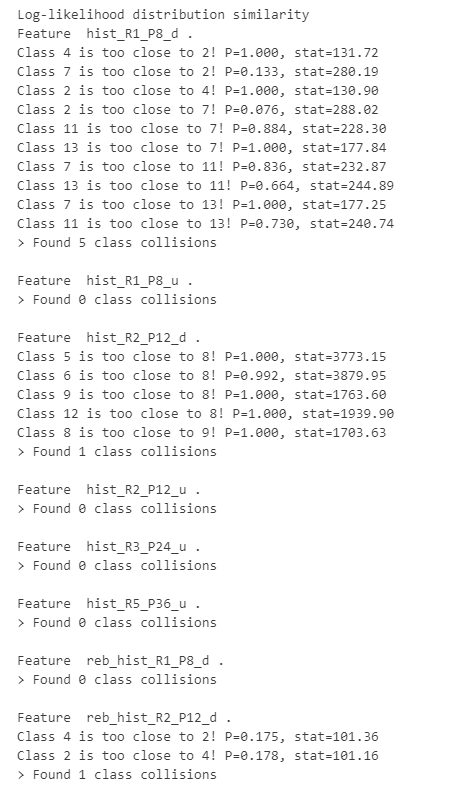
\includegraphics[width=0.9\linewidth]{img/distr-sim.png} 
    \caption{
        Результати критерію близькості розподілів для загальної вибірки.
    }
    \label{fig:distr-sim-all}
    \end{subfigure}%
    \hfill
    \begin{subfigure}{0.48\textwidth}
    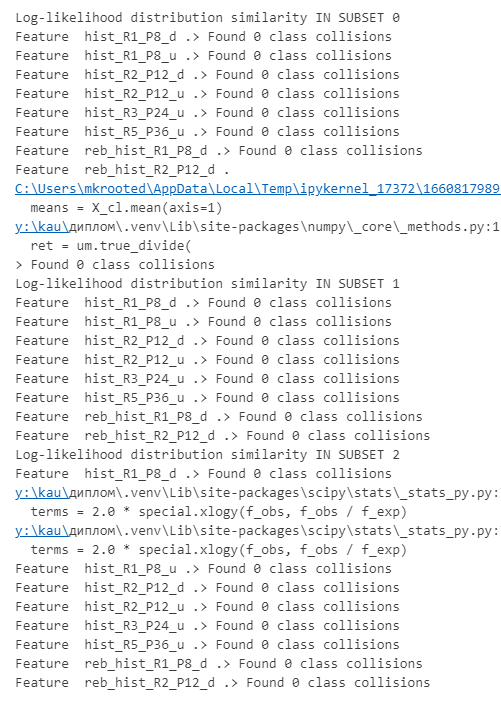
\includegraphics[width=0.9\linewidth]{img/distr-sim-subsets.png}
    \caption{
        Результати критерію близькості розподілів враховуючи зображення, з якого походять патчі. 
    }
    \label{fig:distr-sim-subsets}
    \end{subfigure}
    
    \caption{}
    \label{fig:distr-sim}
\end{figure}

Бачимо, що у загальній вибірці лише стандартні дескриптори R1P8 та R2P12 "плутають" деякі класи; 
проте, це не спостерігається у вибірці, що враховує зображення, з яких походять патчі.
В обох випадках спостерігалися проблеми із нульовими частотами стандартного дескриптора R2P12 через його велику множину значень.
Таким чином, дійсно маємо підстави моделювати текстуру через розподіл значень дескриптора і можемо переходити до класифікації.

\subsection{Класифікація частково відомих текстур}\label{section2.1d}

Побудовано два класифікатора: примітивний класифікатор на основі близькості до середньої гістограми, 
та класифікатор за 3-ма найближчими сусідами із евклідовою метрикою (що грубо еквівалентно статистиці $\chi^2$ близкості розподілів).
Точність класифікації оцінюватимемо як середнє значення точності класифікації кожного класу текстури --
\begin{equation*}
    \text{precision} = \frac{1}{\# S} \sum_{s \in S} \sum_{I : \kappa(I) = s} \frac{\1(g(I) = s)}{\# \{I : \kappa(I) = s\}}
\end{equation*}
де $S$ - множина класів текстури, $g(I)$ - передбачений класифікатором клас, $\kappa(I)$ - дійсний клас. 
Тобто точність обчислюється як частка правильно класифікованих патчів серед усіх патчів.
Для коректних результатів, точність класифікатора перевіряється лише на патчах, яких не було у тренувальній вибірці.
Тренувальна вибірка складається із випадково обраних 60\% патчів із загальної вибірки, не зважаючи на зображення, з якого утворені патчі.
Таким чином класифікатор вчиться і перевіряється на тих самих зображеннях, але різних їх частинах.
Класифікація виконується за кожним дескриптором окремо від інших.

Перший класифікатор побудовано за принципом, описаним у рівнянні \ref{e:gtest-classifier-1}, 
що відповідає пошуку найближчого середнього вектора згідно відстані Кульбака-Ляйблера.
Результати зображені на Рис. \ref{fig:precision-1}.
Найкраще показують себе стандартний LBP R1P8 дескриптор та дескриптори R1P8 й R2P12 із розбитими на інтервали гістограмами, проте не стандартний R2P12.
Об'єднання значень у інтервали підивщило точність класифікації для дескриптора із великою областю значень.
Рівномірні дескриптори в цілому показали гіршу точність класифікації.
Матриці невідповідностей на Рис. \ref{fig:precision-1} показують кількість патчів із класом рядка, які класифіковані класом стовпця. 

\begin{figure}[h]
    \begin{subfigure}{0.5\textwidth}
    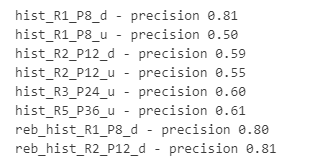
\includegraphics[width=0.95\linewidth]{img/precision-1.png} 
    \caption{
        Точність класифікації за \ref{e:gtest-classifier-1} для різних векторів ознак.
    }
    \end{subfigure}%
    \begin{subfigure}{0.5\textwidth}
    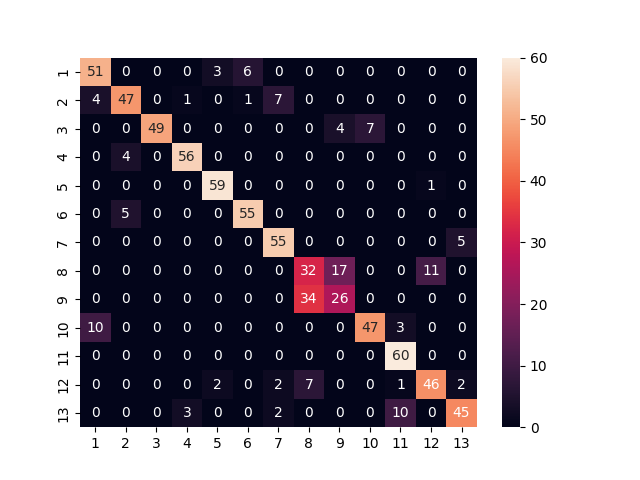
\includegraphics[width=0.95\linewidth]{img/confusion/hist_R1_P8_d.png}
    \caption{
        Матриця невідповідностей стандартного R1P8 (точність 0,81)
    }
    \end{subfigure}

    \begin{subfigure}{0.5\textwidth}
    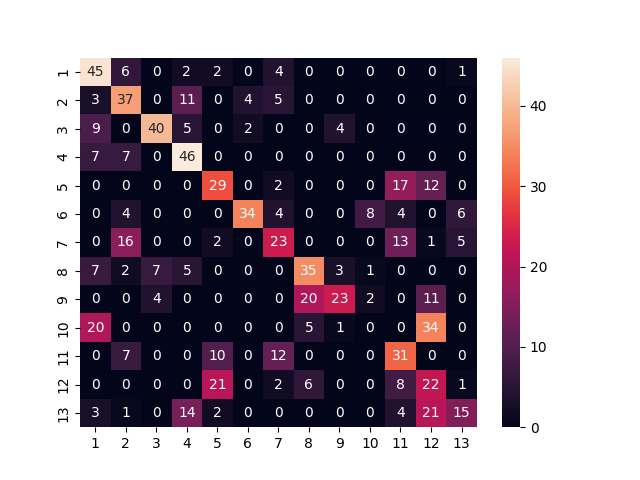
\includegraphics[width=0.95\linewidth]{img/confusion/hist_R1_P8_u.png}
    \caption{
        Матриця невідповідностей рівномірного R1P8 (точність 0,5)
    }
    \end{subfigure}%
    \begin{subfigure}{0.5\textwidth}
    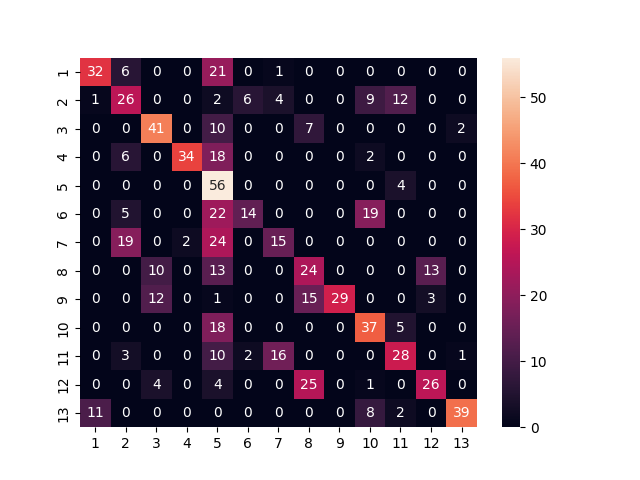
\includegraphics[width=0.95\linewidth]{img/confusion/hist_R5_P36_u.png}
    \caption{
        Матриця невідповідностей рівномірного R5P36 (точність 0,61) 
    }
    \end{subfigure}%
    
    \caption{Класифікатор за близкістю до середнього розподілу}
    \label{fig:precision-1}
\end{figure}

У всіх варіантах спостерігається близькість класів 8 та 9, що відповідають відповідно фотографіям поверхні води та дерев'яного зрізу,
які на око дійсно виглядають дещо схожими. 

Другий класифікатор побудовано на основі \verb|KNeighborsClassifier| з пакету SciPy із стандартною Евклідовою метрикою та трьома сусідами.
Результати зображено на Рис. \ref{fig:precision-2}. 
Точність класифікації з допомогою всіх дескрипторів вийшла досить висока.
Найкраща точність у стандартних дескрипторів R1P8 та R2P12, а
найгірше себе показав рівномірний дескриптор радіуса 5, при цьому будучи точнішим, за всі класифікатори першого типу.
Інші дескриптори призводять до приблизко однаково точної класифікації.

Важливим спостереженням є те, що рівномірні дескриптори використовують суттєво менші вектори ознак 
(не більше 40 координат, порівняно із 256 та 4096 координат для R1P8 та R2P12), 
але породжують всього незначно менш точні класифікатори.
Також цікаво, що KNN класифікатори набагато краще відрізняють навіть візуально схожі класи, які попередній класифікатор розрізняв погано.

\begin{figure}[h]
    \begin{subfigure}{0.5\textwidth}
    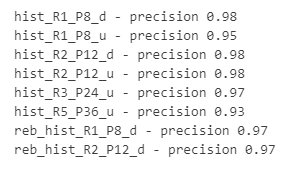
\includegraphics[width=0.95\linewidth]{img/precision-2.png} 
    \caption{
        Точність класифікації за KNN для різних векторів ознак.
    }
    \end{subfigure}%
    \begin{subfigure}{0.5\textwidth}
    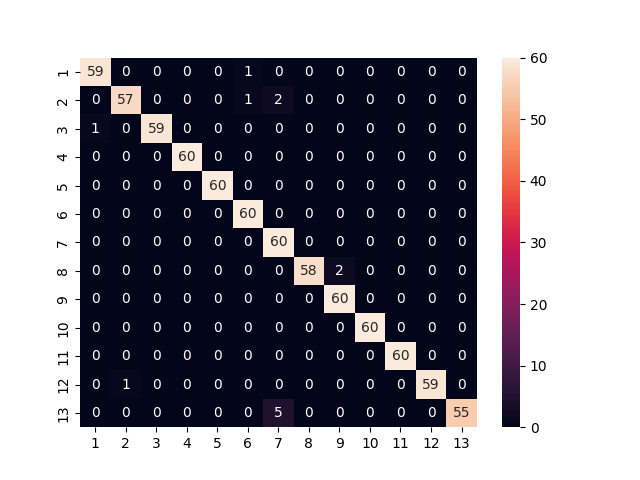
\includegraphics[width=0.95\linewidth]{img/confusion/knn-hist_R1_P8_d.png}
    \caption{
        Матриця невідповідностей стандартного R1P8 (точність 0,98)
    }
    \end{subfigure}

    \begin{subfigure}{0.5\textwidth}
    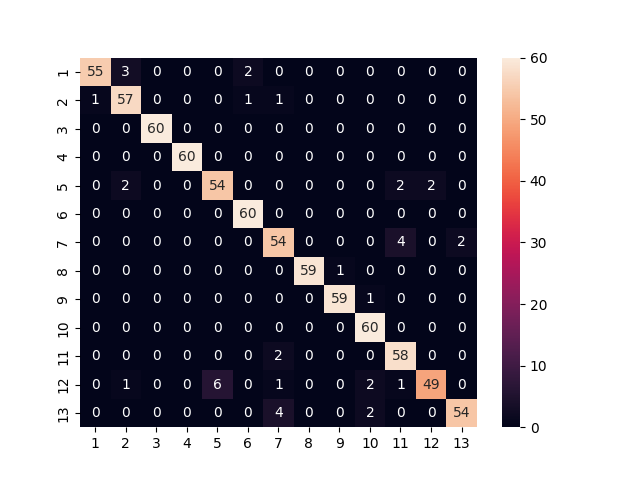
\includegraphics[width=0.95\linewidth]{img/confusion/knn-hist_R1_P8_u.png}
    \caption{
        Матриця невідповідностей рівномірного R1P8 (точність 0,95)
    }
    \end{subfigure}%
    \begin{subfigure}{0.5\textwidth}
    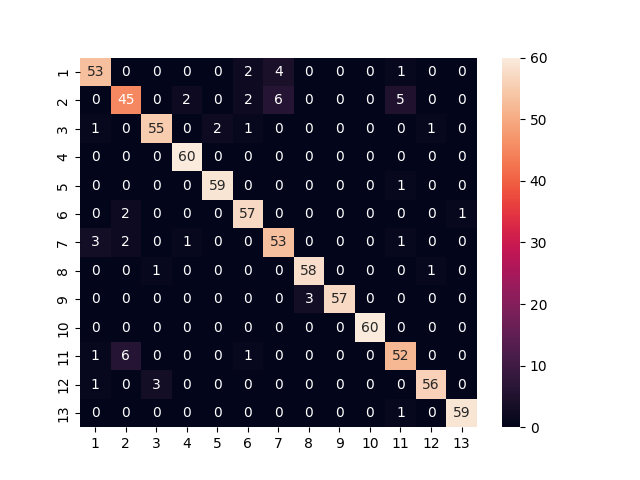
\includegraphics[width=0.95\linewidth]{img/confusion/knn-hist_R5_P36_u.png}
    \caption{
        Матриця невідповідностей рівномірного R5P36 (точність 0,93) 
    }
    \end{subfigure}%
    
    \caption{Класифікатор KNN}
    \label{fig:precision-2}
\end{figure}

\subsection{Класифікація невідомих текстур}\label{section2.1e}
Розділимо патчі за зображеннями, з яких вони походять.
Тренуватимемо класифікатори лише на частині патчів з одного зображення, оцінюватимемо на патчах з іншого.
Таким чином можемо перевірити, наскільки модель з одного представника текстури узагальнюється на інші представники.  
Важливо, що перша та друга фотографії мають однаковий масштаб, проте третя відрізняється масштабом приблизно у 2 рази.
У всіх випадках класифікатор навчається на випадкових 60\% патчах першого зображення, і оцінюється на всіх патчах другого та третього зображень.
Результати зібрано на Рис. \ref{fig:precision-3}.

Бачимо, що для зображень одного масштабу модель досить гарно узагальнюється для обох типів класифікаторів; 
і навіть показує кращий результат, ніж при тренуванні на всіх зображеннях.
З іншого боку, точність на зображенні більшого масштабу зрівнянна із вибором класу випадковим чином ($\frac{1}{13} \approx 0,08$), 
що свідчить про очікувану несумісність навчальних і тестових даних, тобто значну різницю у розподілах дескрипторів.
Цікаво, що найкраще узагальнюються моделі, побудовані на дескрипторах із розбиттям множини значень на інтервали.
Найгірше узагальнювалась модель на основі гістограм дескриптора із найбільшою множиною значень, R2P12.

\begin{figure}[h]
    \begin{subfigure}{0.5\textwidth}
    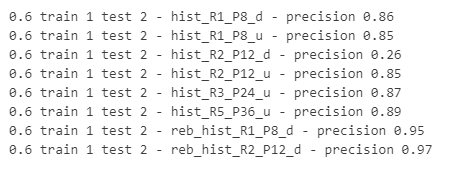
\includegraphics[width=0.95\linewidth]{img/precision-3.png} 
    \caption{
        Класифікатор на середніх гістограмах. Навчено на зображенні 1, перевірено на зображенні 2 того ж масштабу.
    }
    \end{subfigure}%
    \begin{subfigure}{0.5\textwidth}
    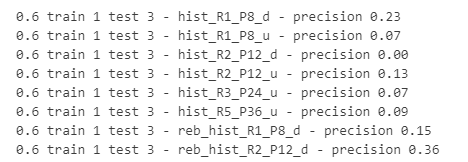
\includegraphics[width=0.95\linewidth]{img/precision-4.png}
    \caption{
        Класифікатор на середніх гістограмах. Навчено на зображенні 1, перевірено на зображенні 3 іншого масштабу.
    }
    \end{subfigure}

    \begin{subfigure}{0.5\textwidth}
    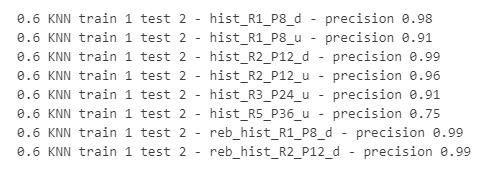
\includegraphics[width=0.95\linewidth]{img/precision-3-knn.png} 
    \caption{
        KNN класифікатор. Навчено на зображенні 1, перевірено на зображенні 2.
    }
    \end{subfigure}%
    \begin{subfigure}{0.5\textwidth}
    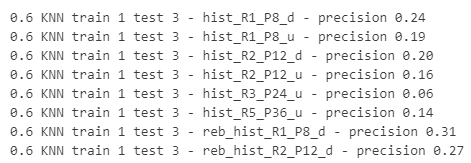
\includegraphics[width=0.95\linewidth]{img/precision-4-knn.png}
    \caption{
        KNN класифікатор. Навчено на зображенні 1, перевірено на зображенні 3.
    }
    \end{subfigure}
    
    \caption{}
    \label{fig:precision-3}
\end{figure}


\subsection{Висновки}\label{section2.1f}

Текстуру дійсно має сенс моделювати як розподіл значень деяких текстурних дескрипторів.
Утворена модель достатньо загальна, щоб описувати і інші реалізації текстури, проте лише схожих масштабів; 
моделі однієї текстури різних масштабів відрізняються.
Рівномірні LBP дескриптори дійсно описують текстуру достатньо повно: за умови правильно підібраного класифікатора, короткі вектори ознак від рівномірних дескрипторів можуть давати точність класифікації 
співставну із значно довшими ознаками від стандартних дескрипторів. 
Гістограми із великою кількістю комірок та великою кількістю малих частот є сенс згруповувати за інтервалами, що також призводить до кращої придатності моделі до узагальнення.
Класифікація за K найближчими сусідами призводила до точнішої класифікації у практично всіх випадках, а особливо у випадку якісно різних представників одного класу текстури.


\section{Розробка пакету fastLBP}\label{section2.2}

Працюючи в лабораторії системної біології SysBio Інституту молекулярної біології та генетики під керівництвом А.О. Фролової 
та у колаборації із університетом Sanger було розроблено програмне забезпечення для ефективного обчислення гістограм 
рівномірних текстурних дескрипторів LBP.
ПЗ оформлено у вигляді пакету Python і доступне публічно через PyPi як \href{https://pypi.org/project/fastlbp-imbg/}{fastlbp-imbg}.
Вихідний код опубліковано у репозиторії \url{https://github.com/imbg-ua/fastLBP} на Github.

\subsection{Опис функціональності}\label{section2.2a}\hfill

Пакет складається з двох принципових частин. 
Перша частина -- це оптимізований код обчислення рівномірних LBP дескрипторів на мові Cython, що компілюється у бінарний модуль Python 
і доступний ззовні як функції \verb|fastlbp_imbg.lbp.uniform_lbp_uint8|, \verb|uniform_lbp_uint8_masked| та подібні.
Модуль розроблено на основі реалізації у пакеті Scikit-Image (\verb|skimage.feature.local_binary_pattern|).
Головними перевагами модуля є в декілька разів менше використання пам'яті, дещо швидше обчислення, і підтримка маскування вхідного масива для 
пропуску частини пікелів.

Друга частина пакету це багатопоточна утиліта обчислення локальних ознак (гістограм) на основі рівномірних LBP дескрипторів із різними параметрами $R$ та $P$.
Ознаки обчислюються для неперетинних патчів зображення визначеного розміру як конкатенація гістограм.
Багатопоточність дає можливість у рази зменшити час обчислення у середовищах із достатньою кількостю процесорів.
Утиліта адаптована для особливостей роботи із великими зображеннями: 
передбачено зберігання проміжних результатів, оптимізовано операції введення-виведення, 
реалізовано кешування для того, щоб уникнути повтору деяких проміжних обчислень.

\subsection{Особливості реалізації дескриптора}\label{section2.2b}\hfill

У реалізації дескриптора в fastLBP підтримується лише рівномірний варіант LBP.
Це дозволило спеціалізувати функцію обчислення LBP коду, позбавитись багатьох перевірок у головному циклі, і уточнити типи даних для вхідних та вихідних масивів.
Основне зменшення використання пам'яті походить від використання \verb|uint16| замість стандартних \verb|float64|, 
і уникнення зайвих копіювань даних у Python-обгортці основної функції.

Для випадків, коли необхідно обчислити ознаки лише частини зображення, розроблено масковані варіанти дескриптора. 
Функція \verb|uniform_lbp_uint8_patch_masked| приймає бінарну маску патчів, які потрібно обчислити, що дозволяє пропускати обчислення пікселів цілими блоками. 

\subsection{Особливості реалізації утиліти обчислення ознак}\label{section2.2c}\hfill

Обчислення ознак розділено на підзадачі за каналами та параметрами $R,P$ і відбувається у декілька етапів.
Спершу для фіксованих $(R,P)$ обчислюються LBP коди фіксованого каналу зображення (або на маскованих частинах зображення).
Далі зображення розділюється на патчі однакового визначеного розміру і обчислюється гістограма значень дескриптора для кожного патча.
Результати записуються у попередньо визначений сегмент файлу на диску.
Структура файлу визначена так, що після запису всіх сегментів утворюється масив конкатенованих гістограм, по одній для кожного патча зображення.
Таким чином ознака патча утворюється як конкатенація гістограм $H_1,\dots ,H_r$ LBP дескрипторів із параметрами $(R_1,P_1),\dots ,(R_r,P_r)$ для кожного каналу зображення 
(спершу всі гістограми одного каналу, потім наступного, і так далі).
Ці ознаки далі успішно використовувалися у задачах сегментації зораження.

Розміри патча можуть бути як більше, так і менше за R.
Важливо, що для коректного обчислення гістограм, недостатньо лише пікселів патча: 
для обчислення LBP кодів пікселів, близьких до межі, необхідні значення пікселів сусідніх патчів.

Для зручності роботи реалізовано кеш значень дескрипторів. 
Це дозволяє пробувати різні версії ознак без потреби обчислювати всі значення дескриптора заново, 
а також допомагає в роботі із великими зображеннями -- обчислення не втрачаються повністю за аварійного переривання роботи утиліти.

\begin{figure}[h]
    \centering
    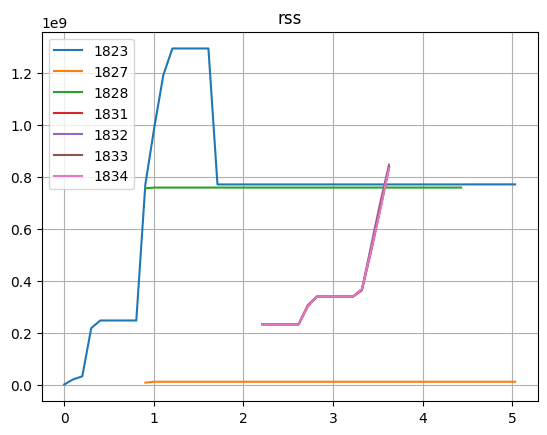
\includegraphics[width=0.5\textwidth]{img/fastlbp/memtest-1-rss.png}
    \caption{
        Типовий профіль використання пам'яті різними підпроцесами утиліти.
    }
    \label{fig:memprofile}
\end{figure}

Впродовж розробки утиліти приділено багато часу оптимізації швидкодії та використання пам'яті. 
На рис.~\ref{fig:memprofile} зображено типовий профіль використання пам'яті підпроцесами.
Особливо виділяються синій материнський процес, що виконує підготовчу роботу і запускає інші; 
та родина дочірніх процесів із поступово зростаючим споживанням.
Поширеними причинами великого споживання пам'яті було некоректне розміщення масивів у пам'яті перед передачею дочірнім процесам 
та копіювання масивів, яке можна уникнути. 

Через багатопоточне обчислення, підбір метрик використання пам'яті та інших метрик ефективності виявився неочевидною задачею.
Також, швидкодія і використання пам'яті багатогранно перевірялися у реальних умовах на обчислювальному кластері Sanger.
Окрім цього, вся ключова функціональність пакету перевіряється автоматичним тестуванням -- від коректності обчислення дескрипторів та очікуваного впливу параметрів обчислення ознак, 
до перевірки дрібних допоміжних функцій і роботи з файловою системою. 

Утиліта стала частиною більшого алгоритму семантичної сегментації гістопатологічних зоображень, 
який було представлено на конференції ECCB 2024 \cite{fastlbp2024}.

\subsection{Оцінка швидкодії}\label{section2.2d}\hfill

Було виконано багатостороннє тестування пакету і оцінка його часу виконання й використання пам'яті, 
а також оцінка залежності цих величин від вхідних параметрів.
Практично підтверджено, що час виконання лінійно залежить від кількості пікселів у зображенні (рис.~\ref{subfig:time-vs-npixels}), 
що вказує на коректність реалізації. Доведено ефективність паралелізації обчислень у певному діапазоні кількості процесорів (рис.~\ref{subfig:parallell-efficiency-a}, рис.~\ref{subfig:parallell-efficiency-b}),
та доцільність використання маски для пропуску частин зображення (рис.~\ref{subfig:parallell-efficiency-с}).
Для надійності, кожен тест швидкодії виконувався декілька разів. На графіку точка вказує на медіану виміряної величини, 
а вертикальний відрізок навколо точки показує розкид між мінімальним та максимальним значеннями.

\begin{figure}[h]
    \begin{subfigure}{0.45\textwidth}
    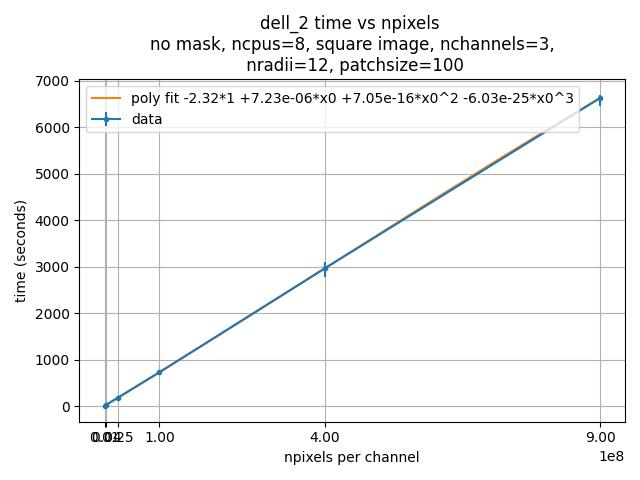
\includegraphics[width=0.99\linewidth]{img/fastlbp/complexity-time_npixels_nc3.jpg}
    \caption{
        Час виконання fastLBP від кількості пікселів.
    }
    \label{subfig:time-vs-npixels}
    \end{subfigure}%
    \begin{subfigure}{0.45\textwidth}
    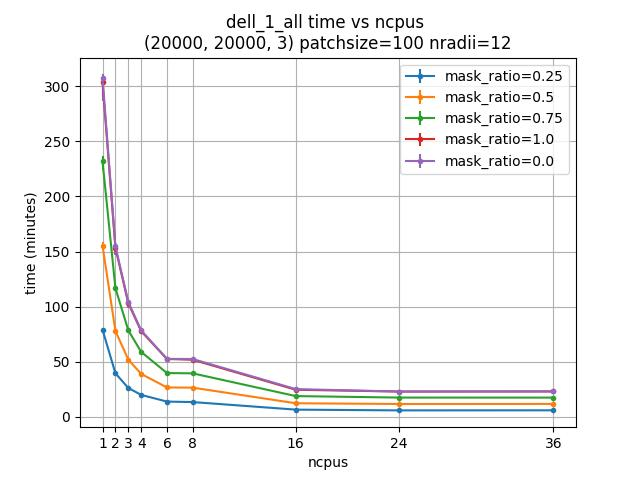
\includegraphics[width=0.99\linewidth]{img/fastlbp/time_ncpus.jpg} 
    \caption{
        Час виконання від кількості процесорів для масок різної площі.
    }
    \label{subfig:parallell-efficiency-a}
    \end{subfigure}

    \begin{subfigure}{0.45\textwidth}
    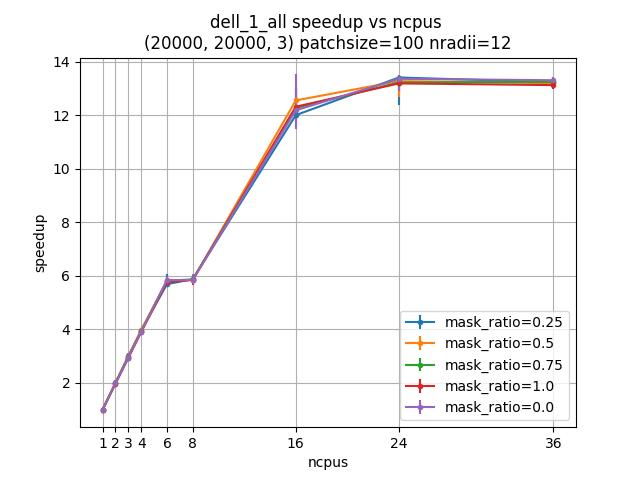
\includegraphics[width=0.99\linewidth]{img/fastlbp/speedup_ncpus.jpg}
    \caption{
        Пришвидшення від кількості процесорів для масок різної площі.
    }
    \label{subfig:parallell-efficiency-b}
    \end{subfigure}%
    \begin{subfigure}{0.45\textwidth}
    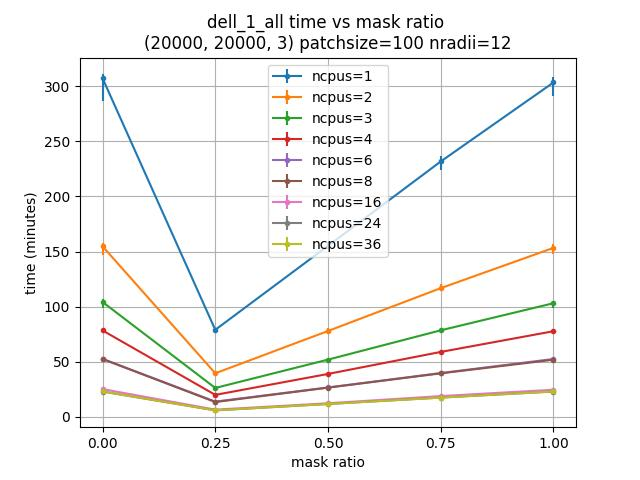
\includegraphics[width=0.99\linewidth]{img/fastlbp/time_mr.jpg}
    \caption{
        Час від площі маски для різних кількостей процесорів.
    }
    \label{subfig:parallell-efficiency-с}
    \end{subfigure}
    
    \caption{Результати оцінки швидкодії.}
    \label{fig:parallell-efficiency}
\end{figure}

\newpage

\phantomsection
\chapter*{Висновки}
\addcontentsline{toc}{chapter}{Висновки}

В роботі описана побудова теорії моделювання текстур через розподіли текстурних дескрипторів,
а також проаналізовано сам дескриптор, його варіанти, і припущення моделі щодо даних.
Коректність теоретичного формулювання та сформульовані припущення підтверджено 
у практичній задачі класифікації текстур.

Продемонстровано, що текстуру доцільно моделювати як розподіл значень дескрипторів LBP на зображенні.
Показано, що утворена з однієї реалізації текстури модель є достатньо загальною, 
щоб описувати і інші реалізації текстури, проте лише схожих масштабів; 
розподіли дескрипторів суттєво відрізняються для зображень різних масштабів.
Наведено підстави вважати, що ``рівномірні'' LBP дескриптори дійсно описують текстуру достатньо повно: 
за умови правильно підібраного класифікатора, короткі вектори ознак від рівномірних дескрипторів можуть 
давати точність класифікації співставну із значно довшими ознаками від стандартних дескрипторів. 

Код практичної частини і статистичних досліджень доступний у відкритому репозиторії \url{https://github.com/mkrooted256/master-thesis}.
Код пакету fastLBP доступний у відкритому репозиторії \url{https://github.com/imbg-ua/fastLBP}.


\newpage

\phantomsection
\renewcommand{\bibname}{Список використаних джерел}

\newpage

\bibliographystyle{plain} %plain %sigma %amsalpha %ugost2008
\addcontentsline{toc}{chapter}{Список використаних джерел}
\bibliography{ref}

% \begin{thebibliography}{99}
% \itemsep=0pt

% % TODO: чому не працює

% \end{thebibliography}

% ДОДАТКИ
% \appendix

% \chapter{Назва додатку}\label{appendix1}

% \section{Назва секції додатку}\label{appendix1.1}

\end{document}



